% Options for packages loaded elsewhere
\PassOptionsToPackage{unicode}{hyperref}
\PassOptionsToPackage{hyphens}{url}
%
\documentclass[
]{article}
\usepackage{amsmath,amssymb}
\usepackage{iftex}
\ifPDFTeX
  \usepackage[T1]{fontenc}
  \usepackage[utf8]{inputenc}
  \usepackage{textcomp} % provide euro and other symbols
\else % if luatex or xetex
  \usepackage{unicode-math} % this also loads fontspec
  \defaultfontfeatures{Scale=MatchLowercase}
  \defaultfontfeatures[\rmfamily]{Ligatures=TeX,Scale=1}
\fi
\usepackage{lmodern}
\ifPDFTeX\else
  % xetex/luatex font selection
\fi
% Use upquote if available, for straight quotes in verbatim environments
\IfFileExists{upquote.sty}{\usepackage{upquote}}{}
\IfFileExists{microtype.sty}{% use microtype if available
  \usepackage[]{microtype}
  \UseMicrotypeSet[protrusion]{basicmath} % disable protrusion for tt fonts
}{}
\makeatletter
\@ifundefined{KOMAClassName}{% if non-KOMA class
  \IfFileExists{parskip.sty}{%
    \usepackage{parskip}
  }{% else
    \setlength{\parindent}{0pt}
    \setlength{\parskip}{6pt plus 2pt minus 1pt}}
}{% if KOMA class
  \KOMAoptions{parskip=half}}
\makeatother
\usepackage{xcolor}
\usepackage[margin=1in]{geometry}
\usepackage{longtable,booktabs,array}
\usepackage{calc} % for calculating minipage widths
% Correct order of tables after \paragraph or \subparagraph
\usepackage{etoolbox}
\makeatletter
\patchcmd\longtable{\par}{\if@noskipsec\mbox{}\fi\par}{}{}
\makeatother
% Allow footnotes in longtable head/foot
\IfFileExists{footnotehyper.sty}{\usepackage{footnotehyper}}{\usepackage{footnote}}
\makesavenoteenv{longtable}
\usepackage{graphicx}
\makeatletter
\def\maxwidth{\ifdim\Gin@nat@width>\linewidth\linewidth\else\Gin@nat@width\fi}
\def\maxheight{\ifdim\Gin@nat@height>\textheight\textheight\else\Gin@nat@height\fi}
\makeatother
% Scale images if necessary, so that they will not overflow the page
% margins by default, and it is still possible to overwrite the defaults
% using explicit options in \includegraphics[width, height, ...]{}
\setkeys{Gin}{width=\maxwidth,height=\maxheight,keepaspectratio}
% Set default figure placement to htbp
\makeatletter
\def\fps@figure{htbp}
\makeatother
\setlength{\emergencystretch}{3em} % prevent overfull lines
\providecommand{\tightlist}{%
  \setlength{\itemsep}{0pt}\setlength{\parskip}{0pt}}
\setcounter{secnumdepth}{-\maxdimen} % remove section numbering
\usepackage{hyperref}
\usepackage{graphicx}
\graphicspath{{stat-tables_files/figure-latex/}}
\usepackage{geometry}
\geometry{a4paper,left=.6in,right=.6in,top=1in,bottom=1in}
\usepackage{booktabs}
\usepackage{longtable}
\usepackage{array}
\usepackage{multirow}
\usepackage{wrapfig}
\usepackage{float}
\usepackage{colortbl}
\usepackage{pdflscape}
\usepackage{tabu}
\usepackage{threeparttable}
\usepackage{threeparttablex}
\usepackage[normalem]{ulem}
\usepackage{makecell}
\usepackage{xcolor}
\ifLuaTeX
  \usepackage{selnolig}  % disable illegal ligatures
\fi
\usepackage{bookmark}
\IfFileExists{xurl.sty}{\usepackage{xurl}}{} % add URL line breaks if available
\urlstyle{same}
\hypersetup{
  hidelinks,
  pdfcreator={LaTeX via pandoc}}

\author{}
\date{\vspace{-2.5em}}

\begin{document}

\thispagestyle{empty}
\begin{center}
~\\
\vspace{2cm}
{\Huge Statistical Tables}
~\\~\\
v1.00 (last updated: 20 Oct 2024)
\vspace{5cm}
\end{center}

\begin{center}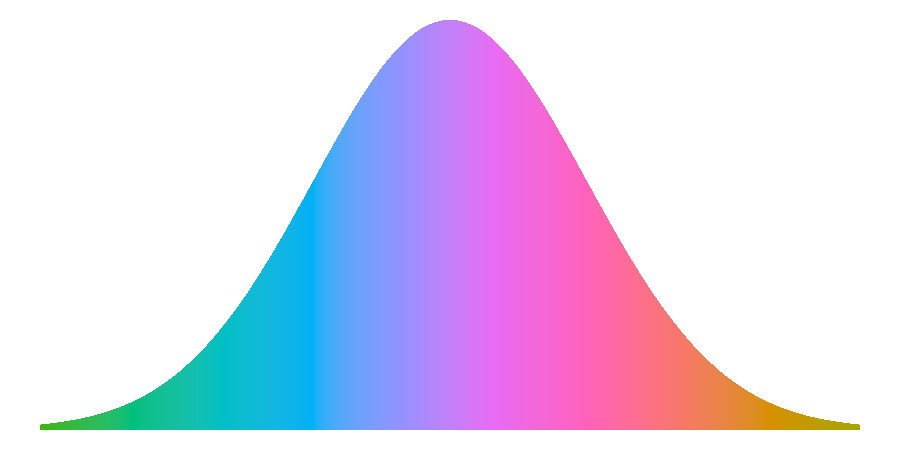
\includegraphics[width=\textwidth]{figure/unnamed-chunk-1-1} \end{center}

\vfill
\begin{center}
Copyright (c) 2024--present SKY-TKP
~\\
\href{https://github.com/SKY-TKP}{\texttt{https://github.com/SKY-TKP}}
\end{center}

\newpage

\subsubsection{Summary some
distribution}\label{summary-some-distribution}

Discrete Probability Distribution

\begin{longtable}[]{@{}
  >{\raggedright\arraybackslash}p{(\columnwidth - 8\tabcolsep) * \real{0.1657}}
  >{\centering\arraybackslash}p{(\columnwidth - 8\tabcolsep) * \real{0.0888}}
  >{\centering\arraybackslash}p{(\columnwidth - 8\tabcolsep) * \real{0.4024}}
  >{\centering\arraybackslash}p{(\columnwidth - 8\tabcolsep) * \real{0.1006}}
  >{\centering\arraybackslash}p{(\columnwidth - 8\tabcolsep) * \real{0.2426}}@{}}
\toprule\noalign{}
\begin{minipage}[b]{\linewidth}\raggedright
\textbf{Distribution}
\end{minipage} & \begin{minipage}[b]{\linewidth}\centering
\textbf{Parameter}
\end{minipage} & \begin{minipage}[b]{\linewidth}\centering
\textbf{Probability mass function; PMF}
\end{minipage} & \begin{minipage}[b]{\linewidth}\centering
\textbf{Expected Value}
\end{minipage} & \begin{minipage}[b]{\linewidth}\centering
\textbf{Variance}
\end{minipage} \\
\midrule\noalign{}
\endhead
\bottomrule\noalign{}
\endlastfoot
Uniform & \(a, b\) & \(\frac{1}{b - a + 1}\) & \(\frac{a+b}{2}\) &
\(\frac{(b-a+1)^2-1}{12}\) \\
Binomial & \(n, p\) & \(\binom{n}{k}p^k\ (1-p)^k\) & \(np\) & \(npq\) \\
Poisson & \(\lambda\) & \(\frac{e^{-\lambda}{\lambda}^x}{x!}\) &
\(\lambda\) & \(\lambda\) \\
Geometric & \(p\) & \((1-p)^{k-1}p\) & \(\frac{1}{p}\) &
\(\frac{1-p}{p^2}\) \\
Hypergeometric & \(M, N, n\) &
\(\frac{{M \choose k} {N-M \choose n-k}}{{N \choose n}}\) &
\(n \frac{M}{N}\) &
\(n \frac{M}{N} \left(1-\frac{M}{N}\right) \frac{N-n}{N-1}\) \\
Negative Binomial & \(r, p\) & \({k-1 \choose r-1} p^r (1-p)^{k-r}\) &
\(\frac{r}{p}\) & \(\frac{r(1-p)}{p^2}\) \\
\end{longtable}

Continuous Probability Distribution

\begin{longtable}[]{@{}
  >{\raggedright\arraybackslash}p{(\columnwidth - 8\tabcolsep) * \real{0.1380}}
  >{\centering\arraybackslash}p{(\columnwidth - 8\tabcolsep) * \real{0.5354}}
  >{\centering\arraybackslash}p{(\columnwidth - 8\tabcolsep) * \real{0.0875}}
  >{\centering\arraybackslash}p{(\columnwidth - 8\tabcolsep) * \real{0.1919}}
  >{\centering\arraybackslash}p{(\columnwidth - 8\tabcolsep) * \real{0.0471}}@{}}
\toprule\noalign{}
\begin{minipage}[b]{\linewidth}\raggedright
\textbf{Distribution}
\end{minipage} & \begin{minipage}[b]{\linewidth}\centering
\textbf{Probability density function; PDF}
\end{minipage} & \begin{minipage}[b]{\linewidth}\centering
\textbf{Expected Value}
\end{minipage} & \begin{minipage}[b]{\linewidth}\centering
\textbf{Variance}
\end{minipage} & \begin{minipage}[b]{\linewidth}\centering
\textbf{Note}
\end{minipage} \\
\midrule\noalign{}
\endhead
\bottomrule\noalign{}
\endlastfoot
Uniform & \(\frac{1}{b - a}\) & \(\frac{a+b}{2}\) &
\(\frac{(b-a)^2}{12}\) & - \\
Normal &
\(\frac{1}{\sigma\sqrt{2\pi}}e^{ -\frac{1}{2}\left(\frac{x-\mu}{\sigma}\right)^{\!2}}\)
& \(\mu\) & \(\sigma\) & - \\
Z (Standard Normal) & \(\frac{1}{\sqrt{2\pi}}e^{-\frac{1}{2}z^{\!2}}\) &
0 & 1 & - \\
Exponential & \({\lambda}{e^{-{\lambda}x}}\) & \(\frac{1}{\lambda}\) &
\(\frac{1}{\lambda^2}\) & - \\
Erlang & \(\frac{\lambda^k x^{k-1} e^{-\lambda x}}{(k-1)!}\) &
\(\frac{k}{\lambda}\) & \(\frac{k}{\lambda^2}\) & \\
Chi-squared & \(\frac{1}{2^{n/2}\Gamma(n/2)}x^{(n/2)-1}e^{-x/2}\) &
\(n\) & \(2n\) & \(df\) \\
Student's T &
\(\frac{\Gamma((n+1)/2)}{\sqrt{\pi n}\,\Gamma(n/2)}\left(1+\frac{t^2}{n}\right)^{-\frac{n+1}{2}}\)
& 0 & \(\frac{n}{n-2}\) & \(df\) \\
F-distribution &
\(\frac{\Gamma((n_1+n_2)/2)}{\Gamma(n_1/2)\Gamma(n_2/2)}\left(\frac{n_1}{n_2}\right)^{n_1/2}x^{(n_1/2)-1}\left(1+\frac{n_1}{n_2}x\right)^{-\frac{n_1+n_2}{2}}\)
& \(\frac{n_2}{n_2 - 2}\) &
\(\frac{2n_2^2(n_1 + n_2 - 2)}{n_1(n_2 - 2)^2(n_2 - 4)}\) &
\(df_1, df_2\) \\
Gamma &
\(\frac{\lambda^{\alpha} x^{\alpha - 1} e^{-\lambda x}}{\Gamma(\alpha)}\)
& \(\frac{\alpha}{\lambda}\) & \(\frac{\alpha}{\lambda^2}\) & - \\
\end{longtable}

\newpage

\subsubsection{Summary some distribution -
cont.}\label{summary-some-distribution---cont.}

\begin{longtable}[]{@{}
  >{\raggedright\arraybackslash}p{(\columnwidth - 6\tabcolsep) * \real{0.2778}}
  >{\raggedright\arraybackslash}p{(\columnwidth - 6\tabcolsep) * \real{0.1667}}
  >{\raggedright\arraybackslash}p{(\columnwidth - 6\tabcolsep) * \real{0.2778}}
  >{\centering\arraybackslash}p{(\columnwidth - 6\tabcolsep) * \real{0.2778}}@{}}
\toprule\noalign{}
\begin{minipage}[b]{\linewidth}\raggedright
\textbf{Distribution}
\end{minipage} & \begin{minipage}[b]{\linewidth}\raggedright
\textbf{Notation}
\end{minipage} & \begin{minipage}[b]{\linewidth}\raggedright
\textbf{Domain}
\end{minipage} & \begin{minipage}[b]{\linewidth}\centering
\textbf{Moment Generating Function; MGF}
\end{minipage} \\
\midrule\noalign{}
\endhead
\bottomrule\noalign{}
\endlastfoot
\textbf{Discrete Distributions} & & & \\
Uniform discrete & \(Uniform(a, b)\) & \(\{a, a+1, ..., b\}\) &
\(\frac{e^{at}-e^{bt}}{t(b-a)}\) \\
Binomial & \(Bin(n, p)\) & \(\{0, 1, 2, ..., n\}\) & \((pe^t + q)^n\), q
= 1-p \\
Poisson & \(Poi(\lambda)\) & \(\{0, 1, 2, ...\}\) &
\(e^{\lambda(e^t-1)}\) \\
Geometric & \(Geo(p)\) & \(\{1, 2, 3, ...\}\) & \(\frac{pe^t}{1-qe^t}\),
q = 1-p \\
Hypergeometric & \(Hyper(M,N,k)\) & \(\{0, 1, 2, ..., min(K, n)\}\) &
- \\
Negative binomial & \(NB(r, p)\) & \(\{0, 1, 2, ...\}\) &
\((\frac{pe^t}{1-qe^t})^r\), q = 1-p \\
\textbf{Continuous Distributions} & & & \\
Uniform continuous & \(Uniform(a, b)\) & \([a, b]\) &
\(\frac{e^{bt}-e^{at}}{t(b-a)}\) \\
Normal & \(Normal(\mu, \sigma^2)\) & \((-\infty, \infty)\) &
\(e^{{\mu}t + \frac{1}{2}\sigma^2t^2}\) \\
Z (Standard Normal) & \(Z(0, 1)\) & \((-\infty, \infty)\) &
\(e^{\frac{1}{2}t^2}\) \\
Exponential & \(Expo(\lambda)\) & \([0, \infty)\) &
\(\frac{\lambda}{\lambda-t}\), t \textless{} \(\lambda\) \\
Erlang & Er(\(k,\ \lambda\)) & \([0, \infty)\) and \(k = 0, 1, 2, ..\) &
\((\frac{\lambda}{\lambda-t})^k\), t \textless{} \(\lambda\) \\
Chi-squared & \(\chi^2(n)\) & \([0, \infty)\) &
\((1-2t)^{-\frac{n-1}{2}}\), t \textless{} \(\frac{1}{2}\) \\
Student's t & \(T(n)\) & \((-\infty, \infty)\) & - \\
F-distribution & \(F(n_1, n_2)\) & \([0, \infty)\) & - \\
Gamma & \(Gamma(\alpha,\ \lambda)\) & \([0, \infty)\) &
\((1-\beta t)^{-\alpha}\), t \textless{}\(\frac{1}{\beta}\) \\
\end{longtable}

\newpage

\subsubsection{Table 1: Cumulative probabilities of the standard normal
distribution.}\label{table-1-cumulative-probabilities-of-the-standard-normal-distribution.}

Each table entry is the area \(\alpha\) under the standard normal curve
from \(-\infty\) to \(z(\alpha)\). That is, the entries are
\(\int_{-\infty}^{z(\alpha)}f_Z(z) \, dz = \alpha\), where \(f_Z\) is
the pdf of \(Z\sim \text{N}(0,1)\).

\vspace{1em}

\begin{center}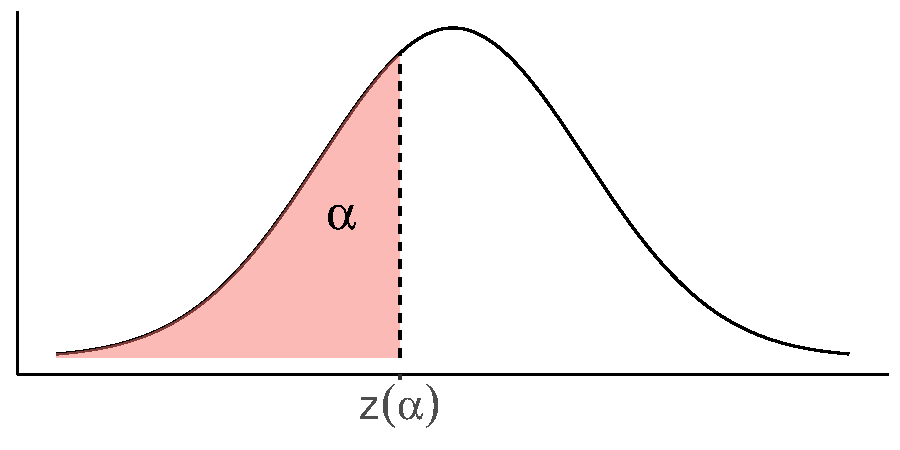
\includegraphics[width=6cm]{figure/unnamed-chunk-2-1} \end{center}

\begin{longtable}[t]{lrrrrrrrrrr}
\toprule
z & .00 & .01 & .02 & .03 & .04 & .05 & .06 & .07 & .08 & .09\\
\midrule
-3.4 & 0.0002 & 0.0003 & 0.0003 & 0.0003 & 0.0003 & 0.0003 & 0.0003 & 0.0003 & 0.0003 & 0.0003\\
-3.3 & 0.0003 & 0.0004 & 0.0004 & 0.0004 & 0.0004 & 0.0004 & 0.0004 & 0.0005 & 0.0005 & 0.0005\\
-3.2 & 0.0005 & 0.0005 & 0.0005 & 0.0006 & 0.0006 & 0.0006 & 0.0006 & 0.0006 & 0.0007 & 0.0007\\
-3.1 & 0.0007 & 0.0007 & 0.0008 & 0.0008 & 0.0008 & 0.0008 & 0.0009 & 0.0009 & 0.0009 & 0.0010\\
-3.0 & 0.0010 & 0.0010 & 0.0011 & 0.0011 & 0.0011 & 0.0012 & 0.0012 & 0.0013 & 0.0013 & 0.0013\\
\addlinespace
-2.9 & 0.0014 & 0.0014 & 0.0015 & 0.0015 & 0.0016 & 0.0016 & 0.0017 & 0.0018 & 0.0018 & 0.0019\\
-2.8 & 0.0019 & 0.0020 & 0.0021 & 0.0021 & 0.0022 & 0.0023 & 0.0023 & 0.0024 & 0.0025 & 0.0026\\
-2.7 & 0.0026 & 0.0027 & 0.0028 & 0.0029 & 0.0030 & 0.0031 & 0.0032 & 0.0033 & 0.0034 & 0.0035\\
-2.6 & 0.0036 & 0.0037 & 0.0038 & 0.0039 & 0.0040 & 0.0041 & 0.0043 & 0.0044 & 0.0045 & 0.0047\\
-2.5 & 0.0048 & 0.0049 & 0.0051 & 0.0052 & 0.0054 & 0.0055 & 0.0057 & 0.0059 & 0.0060 & 0.0062\\
\addlinespace
-2.4 & 0.0064 & 0.0066 & 0.0068 & 0.0069 & 0.0071 & 0.0073 & 0.0075 & 0.0078 & 0.0080 & 0.0082\\
-2.3 & 0.0084 & 0.0087 & 0.0089 & 0.0091 & 0.0094 & 0.0096 & 0.0099 & 0.0102 & 0.0104 & 0.0107\\
-2.2 & 0.0110 & 0.0113 & 0.0116 & 0.0119 & 0.0122 & 0.0125 & 0.0129 & 0.0132 & 0.0136 & 0.0139\\
-2.1 & 0.0143 & 0.0146 & 0.0150 & 0.0154 & 0.0158 & 0.0162 & 0.0166 & 0.0170 & 0.0174 & 0.0179\\
-2.0 & 0.0183 & 0.0188 & 0.0192 & 0.0197 & 0.0202 & 0.0207 & 0.0212 & 0.0217 & 0.0222 & 0.0228\\
\addlinespace
-1.9 & 0.0233 & 0.0239 & 0.0244 & 0.0250 & 0.0256 & 0.0262 & 0.0268 & 0.0274 & 0.0281 & 0.0287\\
-1.8 & 0.0294 & 0.0301 & 0.0307 & 0.0314 & 0.0322 & 0.0329 & 0.0336 & 0.0344 & 0.0351 & 0.0359\\
-1.7 & 0.0367 & 0.0375 & 0.0384 & 0.0392 & 0.0401 & 0.0409 & 0.0418 & 0.0427 & 0.0436 & 0.0446\\
-1.6 & 0.0455 & 0.0465 & 0.0475 & 0.0485 & 0.0495 & 0.0505 & 0.0516 & 0.0526 & 0.0537 & 0.0548\\
-1.5 & 0.0559 & 0.0571 & 0.0582 & 0.0594 & 0.0606 & 0.0618 & 0.0630 & 0.0643 & 0.0655 & 0.0668\\
\addlinespace
-1.4 & 0.0681 & 0.0694 & 0.0708 & 0.0721 & 0.0735 & 0.0749 & 0.0764 & 0.0778 & 0.0793 & 0.0808\\
-1.3 & 0.0823 & 0.0838 & 0.0853 & 0.0869 & 0.0885 & 0.0901 & 0.0918 & 0.0934 & 0.0951 & 0.0968\\
-1.2 & 0.0985 & 0.1003 & 0.1020 & 0.1038 & 0.1056 & 0.1075 & 0.1093 & 0.1112 & 0.1131 & 0.1151\\
-1.1 & 0.1170 & 0.1190 & 0.1210 & 0.1230 & 0.1251 & 0.1271 & 0.1292 & 0.1314 & 0.1335 & 0.1357\\
-1.0 & 0.1379 & 0.1401 & 0.1423 & 0.1446 & 0.1469 & 0.1492 & 0.1515 & 0.1539 & 0.1562 & 0.1587\\
\addlinespace
-0.9 & 0.1611 & 0.1635 & 0.1660 & 0.1685 & 0.1711 & 0.1736 & 0.1762 & 0.1788 & 0.1814 & 0.1841\\
-0.8 & 0.1867 & 0.1894 & 0.1922 & 0.1949 & 0.1977 & 0.2005 & 0.2033 & 0.2061 & 0.2090 & 0.2119\\
-0.7 & 0.2148 & 0.2177 & 0.2206 & 0.2236 & 0.2266 & 0.2296 & 0.2327 & 0.2358 & 0.2389 & 0.2420\\
-0.6 & 0.2451 & 0.2483 & 0.2514 & 0.2546 & 0.2578 & 0.2611 & 0.2643 & 0.2676 & 0.2709 & 0.2743\\
-0.5 & 0.2776 & 0.2810 & 0.2843 & 0.2877 & 0.2912 & 0.2946 & 0.2981 & 0.3015 & 0.3050 & 0.3085\\
\addlinespace
-0.4 & 0.3121 & 0.3156 & 0.3192 & 0.3228 & 0.3264 & 0.3300 & 0.3336 & 0.3372 & 0.3409 & 0.3446\\
-0.3 & 0.3483 & 0.3520 & 0.3557 & 0.3594 & 0.3632 & 0.3669 & 0.3707 & 0.3745 & 0.3783 & 0.3821\\
-0.2 & 0.3859 & 0.3897 & 0.3936 & 0.3974 & 0.4013 & 0.4052 & 0.4090 & 0.4129 & 0.4168 & 0.4207\\
-0.1 & 0.4247 & 0.4286 & 0.4325 & 0.4364 & 0.4404 & 0.4443 & 0.4483 & 0.4522 & 0.4562 & 0.4602\\
0.0 & 0.4641 & 0.4681 & 0.4721 & 0.4761 & 0.4801 & 0.4840 & 0.4880 & 0.4920 & 0.4960 & 0.5000\\
\bottomrule
\end{longtable}

\newpage

\subsubsection{\texorpdfstring{Table 2: Percentiles of the
\(\chi^2\)-distribution.}{Table 2: Percentiles of the \textbackslash chi\^{}2-distribution.}}\label{table-2-percentiles-of-the-chi2-distribution.}

Each table entry is \(\chi^2_k(\alpha)\), where
\(\int_{\chi^2_k(\alpha)}^{\infty}f_X(x) \, dx = \alpha\) with
\(X\sim\chi^2_k\).

\begin{center}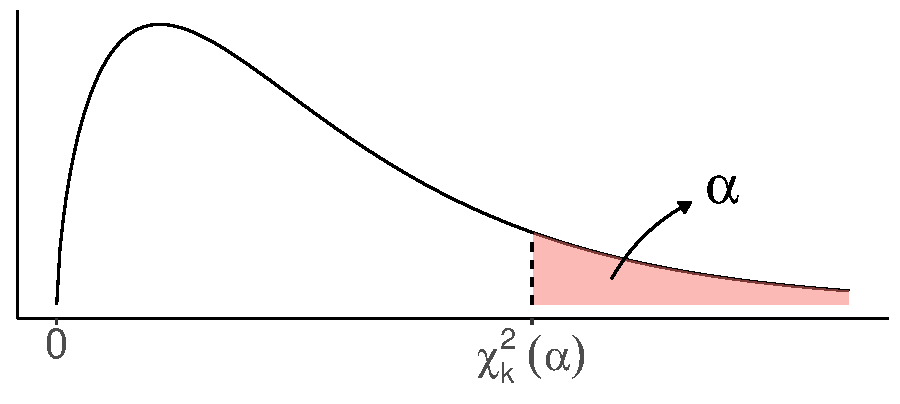
\includegraphics[width=6cm]{figure/unnamed-chunk-3-1} \end{center}

\begin{longtable}[t]{lrrrrrrrrrrr}
\toprule
\multicolumn{1}{c}{ } & \multicolumn{11}{c}{$Area$} \\
\cmidrule(l{3pt}r{3pt}){2-12}
k & 0.005 & 0.010 & 0.025 & 0.050 & 0.100 & 0.500 & 0.900 & 0.950 & 0.975 & 0.990 & 0.995\\
\midrule
1 & 7.879 & 6.635 & 5.024 & 3.841 & 2.706 & 0.455 & 0.016 & 0.004 & 0.001 & 0.000 & 0.000\\
2 & 10.597 & 9.210 & 7.378 & 5.991 & 4.605 & 1.386 & 0.211 & 0.103 & 0.051 & 0.020 & 0.010\\
3 & 12.838 & 11.345 & 9.348 & 7.815 & 6.251 & 2.366 & 0.584 & 0.352 & 0.216 & 0.115 & 0.072\\
4 & 14.860 & 13.277 & 11.143 & 9.488 & 7.779 & 3.357 & 1.064 & 0.711 & 0.484 & 0.297 & 0.207\\
5 & 16.750 & 15.086 & 12.833 & 11.070 & 9.236 & 4.351 & 1.610 & 1.145 & 0.831 & 0.554 & 0.412\\
\addlinespace
6 & 18.548 & 16.812 & 14.449 & 12.592 & 10.645 & 5.348 & 2.204 & 1.635 & 1.237 & 0.872 & 0.676\\
7 & 20.278 & 18.475 & 16.013 & 14.067 & 12.017 & 6.346 & 2.833 & 2.167 & 1.690 & 1.239 & 0.989\\
8 & 21.955 & 20.090 & 17.535 & 15.507 & 13.362 & 7.344 & 3.490 & 2.733 & 2.180 & 1.646 & 1.344\\
9 & 23.589 & 21.666 & 19.023 & 16.919 & 14.684 & 8.343 & 4.168 & 3.325 & 2.700 & 2.088 & 1.735\\
10 & 25.188 & 23.209 & 20.483 & 18.307 & 15.987 & 9.342 & 4.865 & 3.940 & 3.247 & 2.558 & 2.156\\
\addlinespace
11 & 26.757 & 24.725 & 21.920 & 19.675 & 17.275 & 10.341 & 5.578 & 4.575 & 3.816 & 3.053 & 2.603\\
12 & 28.300 & 26.217 & 23.337 & 21.026 & 18.549 & 11.340 & 6.304 & 5.226 & 4.404 & 3.571 & 3.074\\
13 & 29.819 & 27.688 & 24.736 & 22.362 & 19.812 & 12.340 & 7.042 & 5.892 & 5.009 & 4.107 & 3.565\\
14 & 31.319 & 29.141 & 26.119 & 23.685 & 21.064 & 13.339 & 7.790 & 6.571 & 5.629 & 4.660 & 4.075\\
15 & 32.801 & 30.578 & 27.488 & 24.996 & 22.307 & 14.339 & 8.547 & 7.261 & 6.262 & 5.229 & 4.601\\
\addlinespace
16 & 34.267 & 32.000 & 28.845 & 26.296 & 23.542 & 15.338 & 9.312 & 7.962 & 6.908 & 5.812 & 5.142\\
17 & 35.718 & 33.409 & 30.191 & 27.587 & 24.769 & 16.338 & 10.085 & 8.672 & 7.564 & 6.408 & 5.697\\
18 & 37.156 & 34.805 & 31.526 & 28.869 & 25.989 & 17.338 & 10.865 & 9.390 & 8.231 & 7.015 & 6.265\\
19 & 38.582 & 36.191 & 32.852 & 30.144 & 27.204 & 18.338 & 11.651 & 10.117 & 8.907 & 7.633 & 6.844\\
20 & 39.997 & 37.566 & 34.170 & 31.410 & 28.412 & 19.337 & 12.443 & 10.851 & 9.591 & 8.260 & 7.434\\
\addlinespace
21 & 41.401 & 38.932 & 35.479 & 32.671 & 29.615 & 20.337 & 13.240 & 11.591 & 10.283 & 8.897 & 8.034\\
22 & 42.796 & 40.289 & 36.781 & 33.924 & 30.813 & 21.337 & 14.041 & 12.338 & 10.982 & 9.542 & 8.643\\
23 & 44.181 & 41.638 & 38.076 & 35.172 & 32.007 & 22.337 & 14.848 & 13.091 & 11.689 & 10.196 & 9.260\\
24 & 45.559 & 42.980 & 39.364 & 36.415 & 33.196 & 23.337 & 15.659 & 13.848 & 12.401 & 10.856 & 9.886\\
25 & 46.928 & 44.314 & 40.646 & 37.652 & 34.382 & 24.337 & 16.473 & 14.611 & 13.120 & 11.524 & 10.520\\
\addlinespace
26 & 48.290 & 45.642 & 41.923 & 38.885 & 35.563 & 25.336 & 17.292 & 15.379 & 13.844 & 12.198 & 11.160\\
27 & 49.645 & 46.963 & 43.195 & 40.113 & 36.741 & 26.336 & 18.114 & 16.151 & 14.573 & 12.879 & 11.808\\
28 & 50.993 & 48.278 & 44.461 & 41.337 & 37.916 & 27.336 & 18.939 & 16.928 & 15.308 & 13.565 & 12.461\\
29 & 52.336 & 49.588 & 45.722 & 42.557 & 39.087 & 28.336 & 19.768 & 17.708 & 16.047 & 14.256 & 13.121\\
30 & 53.672 & 50.892 & 46.979 & 43.773 & 40.256 & 29.336 & 20.599 & 18.493 & 16.791 & 14.953 & 13.787\\
\addlinespace
40 & 66.766 & 63.691 & 59.342 & 55.758 & 51.805 & 39.335 & 29.051 & 26.509 & 24.433 & 22.164 & 20.707\\
50 & 79.490 & 76.154 & 71.420 & 67.505 & 63.167 & 49.335 & 37.689 & 34.764 & 32.357 & 29.707 & 27.991\\
60 & 91.952 & 88.379 & 83.298 & 79.082 & 74.397 & 59.335 & 46.459 & 43.188 & 40.482 & 37.485 & 35.534\\
70 & 104.215 & 100.425 & 95.023 & 90.531 & 85.527 & 69.334 & 55.329 & 51.739 & 48.758 & 45.442 & 43.275\\
80 & 116.321 & 112.329 & 106.629 & 101.879 & 96.578 & 79.334 & 64.278 & 60.391 & 57.153 & 53.540 & 51.172\\
\addlinespace
90 & 128.299 & 124.116 & 118.136 & 113.145 & 107.565 & 89.334 & 73.291 & 69.126 & 65.647 & 61.754 & 59.196\\
100 & 140.169 & 135.807 & 129.561 & 124.342 & 118.498 & 99.334 & 82.358 & 77.929 & 74.222 & 70.065 & 67.328\\
\bottomrule
\end{longtable}

\newpage

\subsubsection{\texorpdfstring{Table 3: Percentiles of Student's
\(t\)-distribution.}{Table 3: Percentiles of Student's t-distribution.}}\label{table-3-percentiles-of-students-t-distribution.}

Each table entry is \(t_k(\alpha)\), where
\(\int_{t_k(\alpha)}^{\infty}f_X(x) \, dx = \alpha\) with \(X\sim T_k\).

\begin{center}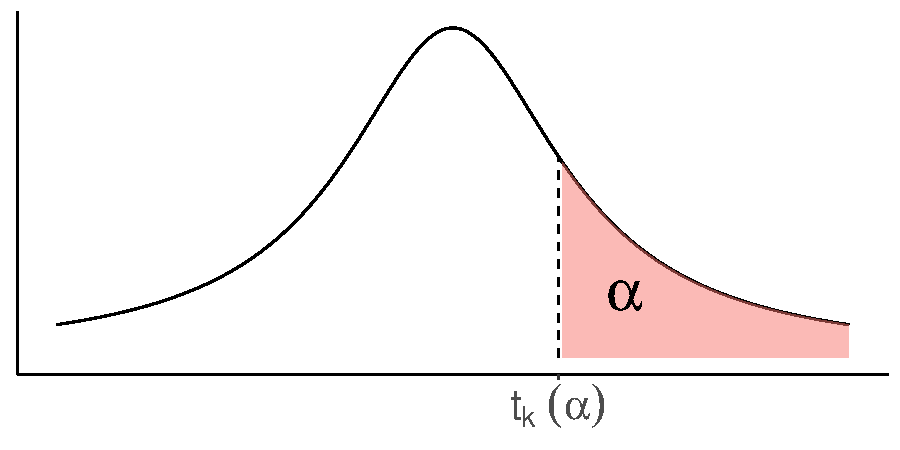
\includegraphics[width=6cm]{figure/unnamed-chunk-4-1} \end{center}

\begin{longtable}[t]{lrrrrrrrrrrrr}
\toprule
\multicolumn{1}{c}{ } & \multicolumn{12}{c}{$Area$} \\
\cmidrule(l{3pt}r{3pt}){2-13}
k & 0.40 & 0.30 & 0.20 & 0.15 & 0.10 & 0.05 & 0.025 & 0.010 & 0.0075 & 0.0050 & 0.0025 & 0.0005\\
\midrule
1 & 0.325 & 0.727 & 1.376 & 1.963 & 3.078 & 6.314 & 12.706 & 31.821 & 42.433 & 63.657 & 127.321 & 636.619\\
2 & 0.289 & 0.617 & 1.061 & 1.386 & 1.886 & 2.920 & 4.303 & 6.965 & 8.073 & 9.925 & 14.089 & 31.599\\
3 & 0.277 & 0.584 & 0.978 & 1.250 & 1.638 & 2.353 & 3.182 & 4.541 & 5.047 & 5.841 & 7.453 & 12.924\\
4 & 0.271 & 0.569 & 0.941 & 1.190 & 1.533 & 2.132 & 2.776 & 3.747 & 4.088 & 4.604 & 5.598 & 8.610\\
5 & 0.267 & 0.559 & 0.920 & 1.156 & 1.476 & 2.015 & 2.571 & 3.365 & 3.634 & 4.032 & 4.773 & 6.869\\
\addlinespace
6 & 0.265 & 0.553 & 0.906 & 1.134 & 1.440 & 1.943 & 2.447 & 3.143 & 3.372 & 3.707 & 4.317 & 5.959\\
7 & 0.263 & 0.549 & 0.896 & 1.119 & 1.415 & 1.895 & 2.365 & 2.998 & 3.203 & 3.499 & 4.029 & 5.408\\
8 & 0.262 & 0.546 & 0.889 & 1.108 & 1.397 & 1.860 & 2.306 & 2.896 & 3.085 & 3.355 & 3.833 & 5.041\\
9 & 0.261 & 0.543 & 0.883 & 1.100 & 1.383 & 1.833 & 2.262 & 2.821 & 2.998 & 3.250 & 3.690 & 4.781\\
10 & 0.260 & 0.542 & 0.879 & 1.093 & 1.372 & 1.812 & 2.228 & 2.764 & 2.932 & 3.169 & 3.581 & 4.587\\
\addlinespace
11 & 0.260 & 0.540 & 0.876 & 1.088 & 1.363 & 1.796 & 2.201 & 2.718 & 2.879 & 3.106 & 3.497 & 4.437\\
12 & 0.259 & 0.539 & 0.873 & 1.083 & 1.356 & 1.782 & 2.179 & 2.681 & 2.836 & 3.055 & 3.428 & 4.318\\
13 & 0.259 & 0.538 & 0.870 & 1.079 & 1.350 & 1.771 & 2.160 & 2.650 & 2.801 & 3.012 & 3.372 & 4.221\\
14 & 0.258 & 0.537 & 0.868 & 1.076 & 1.345 & 1.761 & 2.145 & 2.624 & 2.771 & 2.977 & 3.326 & 4.140\\
15 & 0.258 & 0.536 & 0.866 & 1.074 & 1.341 & 1.753 & 2.131 & 2.602 & 2.746 & 2.947 & 3.286 & 4.073\\
\addlinespace
16 & 0.258 & 0.535 & 0.865 & 1.071 & 1.337 & 1.746 & 2.120 & 2.583 & 2.724 & 2.921 & 3.252 & 4.015\\
17 & 0.257 & 0.534 & 0.863 & 1.069 & 1.333 & 1.740 & 2.110 & 2.567 & 2.706 & 2.898 & 3.222 & 3.965\\
18 & 0.257 & 0.534 & 0.862 & 1.067 & 1.330 & 1.734 & 2.101 & 2.552 & 2.689 & 2.878 & 3.197 & 3.922\\
19 & 0.257 & 0.533 & 0.861 & 1.066 & 1.328 & 1.729 & 2.093 & 2.539 & 2.674 & 2.861 & 3.174 & 3.883\\
20 & 0.257 & 0.533 & 0.860 & 1.064 & 1.325 & 1.725 & 2.086 & 2.528 & 2.661 & 2.845 & 3.153 & 3.850\\
\addlinespace
21 & 0.257 & 0.532 & 0.859 & 1.063 & 1.323 & 1.721 & 2.080 & 2.518 & 2.649 & 2.831 & 3.135 & 3.819\\
22 & 0.256 & 0.532 & 0.858 & 1.061 & 1.321 & 1.717 & 2.074 & 2.508 & 2.639 & 2.819 & 3.119 & 3.792\\
23 & 0.256 & 0.532 & 0.858 & 1.060 & 1.319 & 1.714 & 2.069 & 2.500 & 2.629 & 2.807 & 3.104 & 3.768\\
24 & 0.256 & 0.531 & 0.857 & 1.059 & 1.318 & 1.711 & 2.064 & 2.492 & 2.620 & 2.797 & 3.091 & 3.745\\
25 & 0.256 & 0.531 & 0.856 & 1.058 & 1.316 & 1.708 & 2.060 & 2.485 & 2.612 & 2.787 & 3.078 & 3.725\\
\addlinespace
26 & 0.256 & 0.531 & 0.856 & 1.058 & 1.315 & 1.706 & 2.056 & 2.479 & 2.605 & 2.779 & 3.067 & 3.707\\
27 & 0.256 & 0.531 & 0.855 & 1.057 & 1.314 & 1.703 & 2.052 & 2.473 & 2.598 & 2.771 & 3.057 & 3.690\\
28 & 0.256 & 0.530 & 0.855 & 1.056 & 1.313 & 1.701 & 2.048 & 2.467 & 2.592 & 2.763 & 3.047 & 3.674\\
29 & 0.256 & 0.530 & 0.854 & 1.055 & 1.311 & 1.699 & 2.045 & 2.462 & 2.586 & 2.756 & 3.038 & 3.659\\
30 & 0.256 & 0.530 & 0.854 & 1.055 & 1.310 & 1.697 & 2.042 & 2.457 & 2.581 & 2.750 & 3.030 & 3.646\\
\addlinespace
31 & 0.256 & 0.530 & 0.853 & 1.054 & 1.309 & 1.696 & 2.040 & 2.453 & 2.576 & 2.744 & 3.022 & 3.633\\
32 & 0.255 & 0.530 & 0.853 & 1.054 & 1.309 & 1.694 & 2.037 & 2.449 & 2.571 & 2.738 & 3.015 & 3.622\\
33 & 0.255 & 0.530 & 0.853 & 1.053 & 1.308 & 1.692 & 2.035 & 2.445 & 2.566 & 2.733 & 3.008 & 3.611\\
34 & 0.255 & 0.529 & 0.852 & 1.052 & 1.307 & 1.691 & 2.032 & 2.441 & 2.562 & 2.728 & 3.002 & 3.601\\
35 & 0.255 & 0.529 & 0.852 & 1.052 & 1.306 & 1.690 & 2.030 & 2.438 & 2.558 & 2.724 & 2.996 & 3.591\\
\addlinespace
36 & 0.255 & 0.529 & 0.852 & 1.052 & 1.306 & 1.688 & 2.028 & 2.434 & 2.555 & 2.719 & 2.990 & 3.582\\
37 & 0.255 & 0.529 & 0.851 & 1.051 & 1.305 & 1.687 & 2.026 & 2.431 & 2.551 & 2.715 & 2.985 & 3.574\\
38 & 0.255 & 0.529 & 0.851 & 1.051 & 1.304 & 1.686 & 2.024 & 2.429 & 2.548 & 2.712 & 2.980 & 3.566\\
39 & 0.255 & 0.529 & 0.851 & 1.050 & 1.304 & 1.685 & 2.023 & 2.426 & 2.545 & 2.708 & 2.976 & 3.558\\
40 & 0.255 & 0.529 & 0.851 & 1.050 & 1.303 & 1.684 & 2.021 & 2.423 & 2.542 & 2.704 & 2.971 & 3.551\\
\addlinespace
50 & 0.255 & 0.528 & 0.849 & 1.047 & 1.299 & 1.676 & 2.009 & 2.403 & 2.519 & 2.678 & 2.937 & 3.496\\
60 & 0.254 & 0.527 & 0.848 & 1.045 & 1.296 & 1.671 & 2.000 & 2.390 & 2.504 & 2.660 & 2.915 & 3.460\\
100 & 0.254 & 0.526 & 0.845 & 1.042 & 1.290 & 1.660 & 1.984 & 2.364 & 2.475 & 2.626 & 2.871 & 3.390\\
120 & 0.254 & 0.526 & 0.845 & 1.041 & 1.289 & 1.658 & 1.980 & 2.358 & 2.468 & 2.617 & 2.860 & 3.373\\
Infinity & 0.253 & 0.524 & 0.842 & 1.036 & 1.282 & 1.645 & 1.960 & 2.326 & 2.432 & 2.576 & 2.807 & 3.291\\
\bottomrule
\end{longtable}

\newpage

\subsubsection{\texorpdfstring{Table 4.1: Percentiles of the
\(F\)-distribution.}{Table 4.1: Percentiles of the F-distribution.}}\label{table-4.1-percentiles-of-the-f-distribution.}

Each table entry is
\(F_{k_1,k_2}(\alpha) = F_{k_2,k_1}^{-1}(1-\alpha)\), where
\(\int_{F_{k_1,k_2}(\alpha)}^{{\infty}}f_X(x) \, dx = \alpha\) with
\(X\sim F_{k_1,k_2}\).

\begin{center}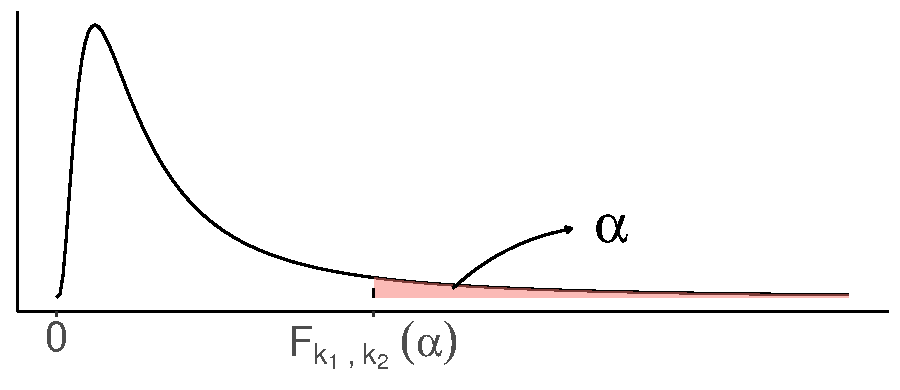
\includegraphics[width=6cm]{figure/unnamed-chunk-5-1} \end{center}

\begin{longtable}[t]{lrrrrrrrrrr}
\toprule
\multicolumn{1}{c}{ } & \multicolumn{10}{c}{$k_1$} \\
\cmidrule(l{3pt}r{3pt}){2-11}
Area & 1 & 2 & 3 & 4 & 5 & 6 & 7 & 8 & 9 & 10\\
\midrule
\addlinespace[0.3em]
\multicolumn{11}{l}{\textbf{$k_2=1$}}\\
\hspace{1em}0.500 & 1.000 & 1.500 & 1.709 & 1.823 & 1.894 & 1.942 & 1.977 & 2.004 & 2.025 & 2.042\\
\hspace{1em}0.100 & 39.86 & 49.50 & 53.59 & 55.83 & 57.24 & 58.20 & 58.91 & 59.44 & 59.86 & 60.19\\
\hspace{1em}0.050 & 161.4 & 199.5 & 215.7 & 224.6 & 230.2 & 234 & 236.8 & 238.9 & 240.5 & 241.9\\
\hspace{1em}0.025 & 647.8 & 799.5 & 864.2 & 899.6 & 921.8 & 937.1 & 948.2 & 956.7 & 963.3 & 968.6\\
\hspace{1em}0.010 & 4052.2 & 4999.5 & 5403.4 & 5624.6 & 5763.6 & 5859 & 5928.4 & 5981.1 & 6022.5 & 6055.8\\
\hspace{1em}0.005 & 16210.7 & 19999.5 & 21614.7 & 22499.6 & 23055.8 & 23437.1 & 23714.6 & 23925.4 & 24091 & 24224.5\\
\hspace{1em}0.001 & 405284.1 & 499999.5 & 540379.2 & 562499.6 & 576404.6 & 585937.1 & 592873.3 & 598144.2 & 602284 & 605621\\
\addlinespace[0.3em]
\multicolumn{11}{l}{\textbf{$k_2=2$}}\\
\hspace{1em}0.500 & 0.667 & 1.000 & 1.135 & 1.207 & 1.252 & 1.282 & 1.305 & 1.321 & 1.334 & 1.345\\
\hspace{1em}0.100 & 8.526 & 9.000 & 9.162 & 9.243 & 9.293 & 9.326 & 9.349 & 9.367 & 9.381 & 9.392\\
\hspace{1em}0.050 & 18.51 & 19.00 & 19.16 & 19.25 & 19.30 & 19.33 & 19.35 & 19.37 & 19.38 & 19.40\\
\hspace{1em}0.025 & 38.51 & 39.00 & 39.17 & 39.25 & 39.30 & 39.33 & 39.36 & 39.37 & 39.39 & 39.40\\
\hspace{1em}0.010 & 98.50 & 99.00 & 99.17 & 99.25 & 99.30 & 99.33 & 99.36 & 99.37 & 99.39 & 99.40\\
\hspace{1em}0.005 & 198.50 & 199.00 & 199.17 & 199.25 & 199.30 & 199.33 & 199.36 & 199.37 & 199.39 & 199.40\\
\hspace{1em}0.001 & 998.50 & 999.00 & 999.17 & 999.25 & 999.30 & 999.33 & 999.36 & 999.37 & 999.39 & 999.40\\
\addlinespace[0.3em]
\multicolumn{11}{l}{\textbf{$k_2=3$}}\\
\hspace{1em}0.500 & 0.585 & 0.881 & 1.000 & 1.063 & 1.102 & 1.129 & 1.148 & 1.163 & 1.174 & 1.183\\
\hspace{1em}0.100 & 5.538 & 5.462 & 5.391 & 5.343 & 5.309 & 5.285 & 5.266 & 5.252 & 5.240 & 5.230\\
\hspace{1em}0.050 & 10.128 & 9.552 & 9.277 & 9.117 & 9.013 & 8.941 & 8.887 & 8.845 & 8.812 & 8.786\\
\hspace{1em}0.025 & 17.44 & 16.04 & 15.44 & 15.10 & 14.88 & 14.73 & 14.62 & 14.54 & 14.47 & 14.42\\
\hspace{1em}0.010 & 34.12 & 30.82 & 29.46 & 28.71 & 28.24 & 27.91 & 27.67 & 27.49 & 27.35 & 27.23\\
\hspace{1em}0.005 & 55.6 & 49.8 & 47.5 & 46.2 & 45.4 & 44.8 & 44.4 & 44.1 & 43.9 & 43.7\\
\hspace{1em}0.001 & 167.0 & 148.5 & 141.1 & 137.1 & 134.6 & 132.8 & 131.6 & 130.6 & 129.9 & 129.2\\
\addlinespace[0.3em]
\multicolumn{11}{l}{\textbf{$k_2=4$}}\\
\hspace{1em}0.500 & 0.549 & 0.828 & 0.941 & 1.000 & 1.037 & 1.062 & 1.080 & 1.093 & 1.104 & 1.113\\
\hspace{1em}0.100 & 4.54 & 4.32 & 4.19 & 4.11 & 4.05 & 4.01 & 3.98 & 3.95 & 3.94 & 3.92\\
\hspace{1em}0.050 & 7.71 & 6.94 & 6.59 & 6.39 & 6.26 & 6.16 & 6.09 & 6.04 & 6.00 & 5.96\\
\hspace{1em}0.025 & 12.22 & 10.65 & 9.98 & 9.60 & 9.36 & 9.20 & 9.07 & 8.98 & 8.90 & 8.84\\
\hspace{1em}0.010 & 21.2 & 18.0 & 16.7 & 16.0 & 15.5 & 15.2 & 15.0 & 14.8 & 14.7 & 14.5\\
\hspace{1em}0.005 & 31.3 & 26.3 & 24.3 & 23.2 & 22.5 & 22.0 & 21.6 & 21.4 & 21.1 & 21.0\\
\hspace{1em}0.001 & 74.1 & 61.2 & 56.2 & 53.4 & 51.7 & 50.5 & 49.7 & 49.0 & 48.5 & 48.1\\
\addlinespace[0.3em]
\multicolumn{11}{l}{\textbf{$k_2=5$}}\\
\hspace{1em}0.500 & 0.528 & 0.799 & 0.907 & 0.965 & 1.000 & 1.024 & 1.041 & 1.055 & 1.065 & 1.073\\
\hspace{1em}0.100 & 4.06 & 3.78 & 3.62 & 3.52 & 3.45 & 3.40 & 3.37 & 3.34 & 3.32 & 3.30\\
\hspace{1em}0.050 & 6.61 & 5.79 & 5.41 & 5.19 & 5.05 & 4.95 & 4.88 & 4.82 & 4.77 & 4.74\\
\hspace{1em}0.025 & 10.01 & 8.43 & 7.76 & 7.39 & 7.15 & 6.98 & 6.85 & 6.76 & 6.68 & 6.62\\
\hspace{1em}0.010 & 16.3 & 13.3 & 12.1 & 11.4 & 11.0 & 10.7 & 10.5 & 10.3 & 10.2 & 10.1\\
\hspace{1em}0.005 & 22.8 & 18.3 & 16.5 & 15.6 & 14.9 & 14.5 & 14.2 & 14.0 & 13.8 & 13.6\\
\hspace{1em}0.001 & 47.2 & 37.1 & 33.2 & 31.1 & 29.8 & 28.8 & 28.2 & 27.6 & 27.2 & 26.9\\
\bottomrule
\end{longtable}

\newpage

\subsubsection{\texorpdfstring{Table 4.2: (Continued) Percentiles of the
\(F\)-distribution.}{Table 4.2: (Continued) Percentiles of the F-distribution.}}\label{table-4.2-continued-percentiles-of-the-f-distribution.}

\begin{longtable}[t]{lrrrrrrrrrr}
\toprule
\multicolumn{1}{c}{ } & \multicolumn{10}{c}{$k_1$} \\
\cmidrule(l{3pt}r{3pt}){2-11}
Area & 11 & 12 & 13 & 14 & 15 & 20 & 30 & 60 & 120 & Infinity\\
\midrule
\addlinespace[0.3em]
\multicolumn{11}{l}{\textbf{$k_2=1$}}\\
\hspace{1em}0.500 & 2.06 & 2.07 & 2.08 & 2.09 & 2.09 & 2.12 & 2.15 & 2.17 & 2.18 & 2.20\\
\hspace{1em}0.100 & 60.5 & 60.7 & 60.9 & 61.1 & 61.2 & 61.7 & 62.3 & 62.8 & 63.1 & 63.3\\
\hspace{1em}0.050 & 243 & 244 & 245 & 245 & 246 & 248 & 250 & 252 & 253 & 254\\
\hspace{1em}0.025 & 973 & 977 & 980 & 983 & 985 & 993 & 1001 & 1010 & 1014 & 1018\\
\hspace{1em}0.010 & 6083 & 6106 & 6126 & 6143 & 6157 & 6209 & 6261 & 6313 & 6339 & 6366\\
\hspace{1em}0.005 & 24334 & 24426 & 24505 & 24572 & 24630 & 24836 & 25044 & 25253 & 25359 & 25464\\
\hspace{1em}0.001 & 608368 & 610668 & 612622 & 614303 & 615764 & 620908 & 626099 & 631337 & 633972 & 636619\\
\addlinespace[0.3em]
\multicolumn{11}{l}{\textbf{$k_2=2$}}\\
\hspace{1em}0.500 & 1.354 & 1.361 & 1.367 & 1.372 & 1.377 & 1.393 & 1.410 & 1.426 & 1.434 & 1.443\\
\hspace{1em}0.100 & 9.401 & 9.408 & 9.415 & 9.420 & 9.425 & 9.441 & 9.458 & 9.475 & 9.483 & 9.491\\
\hspace{1em}0.050 & 19.40 & 19.41 & 19.42 & 19.42 & 19.43 & 19.45 & 19.46 & 19.48 & 19.49 & 19.50\\
\hspace{1em}0.025 & 39.41 & 39.41 & 39.42 & 39.43 & 39.43 & 39.45 & 39.46 & 39.48 & 39.49 & 39.50\\
\hspace{1em}0.010 & 99.41 & 99.42 & 99.42 & 99.43 & 99.43 & 99.45 & 99.47 & 99.48 & 99.49 & 99.50\\
\hspace{1em}0.005 & 199.41 & 199.42 & 199.42 & 199.43 & 199.43 & 199.45 & 199.47 & 199.48 & 199.49 & 199.50\\
\hspace{1em}0.001 & 999.41 & 999.42 & 999.42 & 999.43 & 999.43 & 999.45 & 999.47 & 999.48 & 999.49 & 999.50\\
\addlinespace[0.3em]
\multicolumn{11}{l}{\textbf{$k_2=3$}}\\
\hspace{1em}0.500 & 1.191 & 1.197 & 1.203 & 1.207 & 1.211 & 1.225 & 1.239 & 1.254 & 1.261 & 1.268\\
\hspace{1em}0.100 & 5.222 & 5.216 & 5.210 & 5.205 & 5.200 & 5.184 & 5.168 & 5.151 & 5.143 & 5.134\\
\hspace{1em}0.050 & 8.763 & 8.745 & 8.729 & 8.715 & 8.703 & 8.660 & 8.617 & 8.572 & 8.549 & 8.526\\
\hspace{1em}0.025 & 14.37 & 14.34 & 14.30 & 14.28 & 14.25 & 14.17 & 14.08 & 13.99 & 13.95 & 13.90\\
\hspace{1em}0.010 & 27.13 & 27.05 & 26.98 & 26.92 & 26.87 & 26.69 & 26.50 & 26.32 & 26.22 & 26.13\\
\hspace{1em}0.005 & 43.5 & 43.4 & 43.3 & 43.2 & 43.1 & 42.8 & 42.5 & 42.1 & 42.0 & 41.8\\
\hspace{1em}0.001 & 128.7 & 128.3 & 128.0 & 127.6 & 127.4 & 126.4 & 125.4 & 124.5 & 124.0 & 123.5\\
\addlinespace[0.3em]
\multicolumn{11}{l}{\textbf{$k_2=4$}}\\
\hspace{1em}0.500 & 1.120 & 1.126 & 1.131 & 1.135 & 1.139 & 1.152 & 1.165 & 1.178 & 1.185 & 1.192\\
\hspace{1em}0.100 & 3.91 & 3.90 & 3.89 & 3.88 & 3.87 & 3.84 & 3.82 & 3.79 & 3.78 & 3.76\\
\hspace{1em}0.050 & 5.94 & 5.91 & 5.89 & 5.87 & 5.86 & 5.80 & 5.75 & 5.69 & 5.66 & 5.63\\
\hspace{1em}0.025 & 8.79 & 8.75 & 8.71 & 8.68 & 8.66 & 8.56 & 8.46 & 8.36 & 8.31 & 8.26\\
\hspace{1em}0.010 & 14.5 & 14.4 & 14.3 & 14.2 & 14.2 & 14.0 & 13.8 & 13.7 & 13.6 & 13.5\\
\hspace{1em}0.005 & 20.8 & 20.7 & 20.6 & 20.5 & 20.4 & 20.2 & 19.9 & 19.6 & 19.5 & 19.3\\
\hspace{1em}0.001 & 47.7 & 47.4 & 47.2 & 46.9 & 46.8 & 46.1 & 45.4 & 44.7 & 44.4 & 44.1\\
\addlinespace[0.3em]
\multicolumn{11}{l}{\textbf{$k_2=5$}}\\
\hspace{1em}0.500 & 1.080 & 1.085 & 1.090 & 1.094 & 1.098 & 1.111 & 1.123 & 1.136 & 1.143 & 1.149\\
\hspace{1em}0.100 & 3.28 & 3.27 & 3.26 & 3.25 & 3.24 & 3.21 & 3.17 & 3.14 & 3.12 & 3.10\\
\hspace{1em}0.050 & 4.70 & 4.68 & 4.66 & 4.64 & 4.62 & 4.56 & 4.50 & 4.43 & 4.40 & 4.36\\
\hspace{1em}0.025 & 6.57 & 6.52 & 6.49 & 6.46 & 6.43 & 6.33 & 6.23 & 6.12 & 6.07 & 6.02\\
\hspace{1em}0.010 & 10.0 & 9.9 & 9.8 & 9.8 & 9.7 & 9.6 & 9.4 & 9.2 & 9.1 & 9.0\\
\hspace{1em}0.005 & 13.5 & 13.4 & 13.3 & 13.2 & 13.1 & 12.9 & 12.7 & 12.4 & 12.3 & 12.1\\
\hspace{1em}0.001 & 26.6 & 26.4 & 26.2 & 26.1 & 25.9 & 25.4 & 24.9 & 24.3 & 24.1 & 23.8\\
\bottomrule
\end{longtable}

\newpage

\subsubsection{\texorpdfstring{Table 4.3: (Continued) Percentiles of the
\(F\)-distribution.}{Table 4.3: (Continued) Percentiles of the F-distribution.}}\label{table-4.3-continued-percentiles-of-the-f-distribution.}

\begin{longtable}[t]{lrrrrrrrrrr}
\toprule
\multicolumn{1}{c}{ } & \multicolumn{10}{c}{$k_1$} \\
\cmidrule(l{3pt}r{3pt}){2-11}
Area & 1 & 2 & 3 & 4 & 5 & 6 & 7 & 8 & 9 & 10\\
\midrule
\addlinespace[0.3em]
\multicolumn{11}{l}{\textbf{$k_2=6$}}\\
\hspace{1em}0.500 & 0.515 & 0.780 & 0.886 & 0.942 & 0.977 & 1.000 & 1.017 & 1.030 & 1.040 & 1.048\\
\hspace{1em}0.100 & 3.776 & 3.463 & 3.289 & 3.181 & 3.108 & 3.055 & 3.014 & 2.983 & 2.958 & 2.937\\
\hspace{1em}0.050 & 5.987 & 5.143 & 4.757 & 4.534 & 4.387 & 4.284 & 4.207 & 4.147 & 4.099 & 4.060\\
\hspace{1em}0.025 & 8.813 & 7.260 & 6.599 & 6.227 & 5.988 & 5.820 & 5.695 & 5.600 & 5.523 & 5.461\\
\hspace{1em}0.010 & 13.745 & 10.925 & 9.780 & 9.148 & 8.746 & 8.466 & 8.260 & 8.102 & 7.976 & 7.874\\
\hspace{1em}0.005 & 18.635 & 14.544 & 12.917 & 12.028 & 11.464 & 11.073 & 10.786 & 10.566 & 10.391 & 10.250\\
\hspace{1em}0.001 & 35.507 & 27.000 & 23.703 & 21.924 & 20.803 & 20.030 & 19.463 & 19.030 & 18.688 & 18.411\\
\addlinespace[0.3em]
\multicolumn{11}{l}{\textbf{$k_2=7$}}\\
\hspace{1em}0.500 & 0.506 & 0.767 & 0.871 & 0.926 & 0.960 & 0.983 & 1.000 & 1.013 & 1.022 & 1.030\\
\hspace{1em}0.100 & 3.589 & 3.257 & 3.074 & 2.961 & 2.883 & 2.827 & 2.785 & 2.752 & 2.725 & 2.703\\
\hspace{1em}0.050 & 5.591 & 4.737 & 4.347 & 4.120 & 3.972 & 3.866 & 3.787 & 3.726 & 3.677 & 3.637\\
\hspace{1em}0.025 & 8.073 & 6.542 & 5.890 & 5.523 & 5.285 & 5.119 & 4.995 & 4.899 & 4.823 & 4.761\\
\hspace{1em}0.010 & 12.246 & 9.547 & 8.451 & 7.847 & 7.460 & 7.191 & 6.993 & 6.840 & 6.719 & 6.620\\
\hspace{1em}0.005 & 16.236 & 12.404 & 10.882 & 10.050 & 9.522 & 9.155 & 8.885 & 8.678 & 8.514 & 8.380\\
\hspace{1em}0.001 & 29.245 & 21.689 & 18.772 & 17.198 & 16.206 & 15.521 & 15.019 & 14.634 & 14.330 & 14.083\\
\addlinespace[0.3em]
\multicolumn{11}{l}{\textbf{$k_2=8$}}\\
\hspace{1em}0.500 & 0.499 & 0.757 & 0.860 & 0.915 & 0.948 & 0.971 & 0.988 & 1.000 & 1.010 & 1.018\\
\hspace{1em}0.100 & 3.458 & 3.113 & 2.924 & 2.806 & 2.726 & 2.668 & 2.624 & 2.589 & 2.561 & 2.538\\
\hspace{1em}0.050 & 5.318 & 4.459 & 4.066 & 3.838 & 3.687 & 3.581 & 3.500 & 3.438 & 3.388 & 3.347\\
\hspace{1em}0.025 & 7.571 & 6.059 & 5.416 & 5.053 & 4.817 & 4.652 & 4.529 & 4.433 & 4.357 & 4.295\\
\hspace{1em}0.010 & 11.259 & 8.649 & 7.591 & 7.006 & 6.632 & 6.371 & 6.178 & 6.029 & 5.911 & 5.814\\
\hspace{1em}0.005 & 14.688 & 11.042 & 9.596 & 8.805 & 8.302 & 7.952 & 7.694 & 7.496 & 7.339 & 7.211\\
\hspace{1em}0.001 & 25.415 & 18.494 & 15.829 & 14.392 & 13.485 & 12.858 & 12.398 & 12.046 & 11.767 & 11.540\\
\addlinespace[0.3em]
\multicolumn{11}{l}{\textbf{$k_2=9$}}\\
\hspace{1em}0.500 & 0.494 & 0.749 & 0.852 & 0.906 & 0.939 & 0.962 & 0.978 & 0.990 & 1.000 & 1.008\\
\hspace{1em}0.100 & 3.360 & 3.006 & 2.813 & 2.693 & 2.611 & 2.551 & 2.505 & 2.469 & 2.440 & 2.416\\
\hspace{1em}0.050 & 5.117 & 4.256 & 3.863 & 3.633 & 3.482 & 3.374 & 3.293 & 3.230 & 3.179 & 3.137\\
\hspace{1em}0.025 & 7.209 & 5.715 & 5.078 & 4.718 & 4.484 & 4.320 & 4.197 & 4.102 & 4.026 & 3.964\\
\hspace{1em}0.010 & 10.561 & 8.022 & 6.992 & 6.422 & 6.057 & 5.802 & 5.613 & 5.467 & 5.351 & 5.257\\
\hspace{1em}0.005 & 13.614 & 10.107 & 8.717 & 7.956 & 7.471 & 7.134 & 6.885 & 6.693 & 6.541 & 6.417\\
\hspace{1em}0.001 & 22.857 & 16.387 & 13.902 & 12.560 & 11.714 & 11.128 & 10.698 & 10.368 & 10.107 & 9.894\\
\addlinespace[0.3em]
\multicolumn{11}{l}{\textbf{$k_2=10$}}\\
\hspace{1em}0.500 & 0.490 & 0.743 & 0.845 & 0.899 & 0.932 & 0.954 & 0.971 & 0.983 & 0.992 & 1.000\\
\hspace{1em}0.100 & 3.285 & 2.924 & 2.728 & 2.605 & 2.522 & 2.461 & 2.414 & 2.377 & 2.347 & 2.323\\
\hspace{1em}0.050 & 4.965 & 4.103 & 3.708 & 3.478 & 3.326 & 3.217 & 3.135 & 3.072 & 3.020 & 2.978\\
\hspace{1em}0.025 & 6.937 & 5.456 & 4.826 & 4.468 & 4.236 & 4.072 & 3.950 & 3.855 & 3.779 & 3.717\\
\hspace{1em}0.010 & 10.044 & 7.559 & 6.552 & 5.994 & 5.636 & 5.386 & 5.200 & 5.057 & 4.942 & 4.849\\
\hspace{1em}0.005 & 12.826 & 9.427 & 8.081 & 7.343 & 6.872 & 6.545 & 6.302 & 6.116 & 5.968 & 5.847\\
\hspace{1em}0.001 & 21.040 & 14.905 & 12.553 & 11.283 & 10.481 & 9.926 & 9.517 & 9.204 & 8.956 & 8.754\\
\bottomrule
\end{longtable}

\newpage

\subsubsection{\texorpdfstring{Table 4.4: (Continued) Percentiles of the
\(F\)-distribution.}{Table 4.4: (Continued) Percentiles of the F-distribution.}}\label{table-4.4-continued-percentiles-of-the-f-distribution.}

\begin{longtable}[t]{lrrrrrrrrrr}
\toprule
\multicolumn{1}{c}{ } & \multicolumn{10}{c}{$k_1$} \\
\cmidrule(l{3pt}r{3pt}){2-11}
Area & 11 & 12 & 13 & 14 & 15 & 20 & 30 & 60 & 120 & Infinity\\
\midrule
\addlinespace[0.3em]
\multicolumn{11}{l}{\textbf{$k_2=6$}}\\
\hspace{1em}0.500 & 1.054 & 1.060 & 1.065 & 1.069 & 1.072 & 1.084 & 1.097 & 1.109 & 1.116 & 1.122\\
\hspace{1em}0.100 & 2.920 & 2.905 & 2.892 & 2.881 & 2.871 & 2.836 & 2.800 & 2.762 & 2.742 & 2.722\\
\hspace{1em}0.050 & 4.027 & 4.000 & 3.976 & 3.956 & 3.938 & 3.874 & 3.808 & 3.740 & 3.705 & 3.669\\
\hspace{1em}0.025 & 5.410 & 5.366 & 5.329 & 5.297 & 5.269 & 5.168 & 5.065 & 4.959 & 4.904 & 4.849\\
\hspace{1em}0.010 & 7.790 & 7.718 & 7.657 & 7.605 & 7.559 & 7.396 & 7.229 & 7.057 & 6.969 & 6.880\\
\hspace{1em}0.005 & 10.133 & 10.034 & 9.950 & 9.877 & 9.814 & 9.589 & 9.358 & 9.122 & 9.001 & 8.879\\
\hspace{1em}0.001 & 18.182 & 17.989 & 17.824 & 17.682 & 17.559 & 17.120 & 16.672 & 16.214 & 15.981 & 15.745\\
\addlinespace[0.3em]
\multicolumn{11}{l}{\textbf{$k_2=7$}}\\
\hspace{1em}0.500 & 1.037 & 1.042 & 1.047 & 1.051 & 1.054 & 1.066 & 1.079 & 1.091 & 1.097 & 1.103\\
\hspace{1em}0.100 & 2.684 & 2.668 & 2.654 & 2.643 & 2.632 & 2.595 & 2.555 & 2.514 & 2.493 & 2.471\\
\hspace{1em}0.050 & 3.603 & 3.575 & 3.550 & 3.529 & 3.511 & 3.445 & 3.376 & 3.304 & 3.267 & 3.230\\
\hspace{1em}0.025 & 4.709 & 4.666 & 4.628 & 4.596 & 4.568 & 4.467 & 4.362 & 4.254 & 4.199 & 4.142\\
\hspace{1em}0.010 & 6.538 & 6.469 & 6.410 & 6.359 & 6.314 & 6.155 & 5.992 & 5.824 & 5.737 & 5.650\\
\hspace{1em}0.005 & 8.270 & 8.176 & 8.097 & 8.028 & 7.968 & 7.754 & 7.534 & 7.309 & 7.193 & 7.076\\
\hspace{1em}0.001 & 13.879 & 13.707 & 13.561 & 13.434 & 13.324 & 12.932 & 12.530 & 12.119 & 11.909 & 11.696\\
\addlinespace[0.3em]
\multicolumn{11}{l}{\textbf{$k_2=8$}}\\
\hspace{1em}0.500 & 1.024 & 1.029 & 1.034 & 1.038 & 1.041 & 1.053 & 1.065 & 1.077 & 1.083 & 1.089\\
\hspace{1em}0.100 & 2.519 & 2.502 & 2.488 & 2.475 & 2.464 & 2.425 & 2.383 & 2.339 & 2.316 & 2.293\\
\hspace{1em}0.050 & 3.313 & 3.284 & 3.259 & 3.237 & 3.218 & 3.150 & 3.079 & 3.005 & 2.967 & 2.928\\
\hspace{1em}0.025 & 4.243 & 4.200 & 4.162 & 4.130 & 4.101 & 3.999 & 3.894 & 3.784 & 3.728 & 3.670\\
\hspace{1em}0.010 & 5.734 & 5.667 & 5.609 & 5.559 & 5.515 & 5.359 & 5.198 & 5.032 & 4.946 & 4.859\\
\hspace{1em}0.005 & 7.104 & 7.015 & 6.938 & 6.872 & 6.814 & 6.608 & 6.396 & 6.177 & 6.065 & 5.951\\
\hspace{1em}0.001 & 11.352 & 11.194 & 11.060 & 10.943 & 10.841 & 10.480 & 10.109 & 9.727 & 9.532 & 9.334\\
\addlinespace[0.3em]
\multicolumn{11}{l}{\textbf{$k_2=9$}}\\
\hspace{1em}0.500 & 1.014 & 1.019 & 1.024 & 1.028 & 1.031 & 1.043 & 1.055 & 1.067 & 1.073 & 1.079\\
\hspace{1em}0.100 & 2.396 & 2.379 & 2.364 & 2.351 & 2.340 & 2.298 & 2.255 & 2.208 & 2.184 & 2.159\\
\hspace{1em}0.050 & 3.102 & 3.073 & 3.048 & 3.025 & 3.006 & 2.936 & 2.864 & 2.787 & 2.748 & 2.707\\
\hspace{1em}0.025 & 3.912 & 3.868 & 3.831 & 3.798 & 3.769 & 3.667 & 3.560 & 3.449 & 3.392 & 3.333\\
\hspace{1em}0.010 & 5.178 & 5.111 & 5.055 & 5.005 & 4.962 & 4.808 & 4.649 & 4.483 & 4.398 & 4.311\\
\hspace{1em}0.005 & 6.314 & 6.227 & 6.153 & 6.089 & 6.032 & 5.832 & 5.625 & 5.410 & 5.300 & 5.188\\
\hspace{1em}0.001 & 9.718 & 9.570 & 9.443 & 9.334 & 9.238 & 8.898 & 8.548 & 8.187 & 8.001 & 7.813\\
\addlinespace[0.3em]
\multicolumn{11}{l}{\textbf{$k_2=10$}}\\
\hspace{1em}0.500 & 1.006 & 1.012 & 1.016 & 1.020 & 1.023 & 1.035 & 1.047 & 1.059 & 1.064 & 1.070\\
\hspace{1em}0.100 & 2.302 & 2.284 & 2.269 & 2.255 & 2.244 & 2.201 & 2.155 & 2.107 & 2.082 & 2.055\\
\hspace{1em}0.050 & 2.943 & 2.913 & 2.887 & 2.865 & 2.845 & 2.774 & 2.700 & 2.621 & 2.580 & 2.538\\
\hspace{1em}0.025 & 3.665 & 3.621 & 3.583 & 3.550 & 3.522 & 3.419 & 3.311 & 3.198 & 3.140 & 3.080\\
\hspace{1em}0.010 & 4.772 & 4.706 & 4.650 & 4.601 & 4.558 & 4.405 & 4.247 & 4.082 & 3.996 & 3.909\\
\hspace{1em}0.005 & 5.746 & 5.661 & 5.589 & 5.526 & 5.471 & 5.274 & 5.071 & 4.859 & 4.750 & 4.639\\
\hspace{1em}0.001 & 8.586 & 8.445 & 8.324 & 8.220 & 8.129 & 7.804 & 7.469 & 7.122 & 6.944 & 6.762\\
\bottomrule
\end{longtable}

\newpage

\subsubsection{\texorpdfstring{Table 4.5: (Continued) Percentiles of the
\(F\)-distribution.}{Table 4.5: (Continued) Percentiles of the F-distribution.}}\label{table-4.5-continued-percentiles-of-the-f-distribution.}

\begin{longtable}[t]{lrrrrrrrrrr}
\toprule
\multicolumn{1}{c}{ } & \multicolumn{10}{c}{$k_1$} \\
\cmidrule(l{3pt}r{3pt}){2-11}
Area & 1 & 2 & 3 & 4 & 5 & 6 & 7 & 8 & 9 & 10\\
\midrule
\addlinespace[0.3em]
\multicolumn{11}{l}{\textbf{$k_2=11$}}\\
\hspace{1em}0.500 & 0.486 & 0.739 & 0.840 & 0.893 & 0.926 & 0.948 & 0.964 & 0.977 & 0.986 & 0.994\\
\hspace{1em}0.100 & 3.225 & 2.860 & 2.660 & 2.536 & 2.451 & 2.389 & 2.342 & 2.304 & 2.274 & 2.248\\
\hspace{1em}0.050 & 4.844 & 3.982 & 3.587 & 3.357 & 3.204 & 3.095 & 3.012 & 2.948 & 2.896 & 2.854\\
\hspace{1em}0.025 & 6.724 & 5.256 & 4.630 & 4.275 & 4.044 & 3.881 & 3.759 & 3.664 & 3.588 & 3.526\\
\hspace{1em}0.010 & 9.646 & 7.206 & 6.217 & 5.668 & 5.316 & 5.069 & 4.886 & 4.744 & 4.632 & 4.539\\
\hspace{1em}0.005 & 12.226 & 8.912 & 7.600 & 6.881 & 6.422 & 6.102 & 5.865 & 5.682 & 5.537 & 5.418\\
\hspace{1em}0.001 & 19.687 & 13.812 & 11.561 & 10.346 & 9.578 & 9.047 & 8.655 & 8.355 & 8.116 & 7.922\\
\addlinespace[0.3em]
\multicolumn{11}{l}{\textbf{$k_2=12$}}\\
\hspace{1em}0.500 & 0.484 & 0.735 & 0.835 & 0.888 & 0.921 & 0.943 & 0.959 & 0.972 & 0.981 & 0.989\\
\hspace{1em}0.100 & 3.177 & 2.807 & 2.606 & 2.480 & 2.394 & 2.331 & 2.283 & 2.245 & 2.214 & 2.188\\
\hspace{1em}0.050 & 4.747 & 3.885 & 3.490 & 3.259 & 3.106 & 2.996 & 2.913 & 2.849 & 2.796 & 2.753\\
\hspace{1em}0.025 & 6.554 & 5.096 & 4.474 & 4.121 & 3.891 & 3.728 & 3.607 & 3.512 & 3.436 & 3.374\\
\hspace{1em}0.010 & 9.330 & 6.927 & 5.953 & 5.412 & 5.064 & 4.821 & 4.640 & 4.499 & 4.388 & 4.296\\
\hspace{1em}0.005 & 11.754 & 8.510 & 7.226 & 6.521 & 6.071 & 5.757 & 5.525 & 5.345 & 5.202 & 5.085\\
\hspace{1em}0.001 & 18.643 & 12.974 & 10.804 & 9.633 & 8.892 & 8.379 & 8.001 & 7.710 & 7.480 & 7.292\\
\addlinespace[0.3em]
\multicolumn{11}{l}{\textbf{$k_2=13$}}\\
\hspace{1em}0.500 & 0.481 & 0.731 & 0.832 & 0.885 & 0.917 & 0.939 & 0.955 & 0.967 & 0.977 & 0.984\\
\hspace{1em}0.100 & 3.136 & 2.763 & 2.560 & 2.434 & 2.347 & 2.283 & 2.234 & 2.195 & 2.164 & 2.138\\
\hspace{1em}0.050 & 4.667 & 3.806 & 3.411 & 3.179 & 3.025 & 2.915 & 2.832 & 2.767 & 2.714 & 2.671\\
\hspace{1em}0.025 & 6.414 & 4.965 & 4.347 & 3.996 & 3.767 & 3.604 & 3.483 & 3.388 & 3.312 & 3.250\\
\hspace{1em}0.010 & 9.074 & 6.701 & 5.739 & 5.205 & 4.862 & 4.620 & 4.441 & 4.302 & 4.191 & 4.100\\
\hspace{1em}0.005 & 11.374 & 8.186 & 6.926 & 6.233 & 5.791 & 5.482 & 5.253 & 5.076 & 4.935 & 4.820\\
\hspace{1em}0.001 & 17.815 & 12.313 & 10.209 & 9.073 & 8.354 & 7.856 & 7.489 & 7.206 & 6.982 & 6.799\\
\addlinespace[0.3em]
\multicolumn{11}{l}{\textbf{$k_2=14$}}\\
\hspace{1em}0.500 & 0.479 & 0.729 & 0.828 & 0.881 & 0.914 & 0.936 & 0.952 & 0.964 & 0.973 & 0.981\\
\hspace{1em}0.100 & 3.102 & 2.726 & 2.522 & 2.395 & 2.307 & 2.243 & 2.193 & 2.154 & 2.122 & 2.095\\
\hspace{1em}0.050 & 4.600 & 3.739 & 3.344 & 3.112 & 2.958 & 2.848 & 2.764 & 2.699 & 2.646 & 2.602\\
\hspace{1em}0.025 & 6.298 & 4.857 & 4.242 & 3.892 & 3.663 & 3.501 & 3.380 & 3.285 & 3.209 & 3.147\\
\hspace{1em}0.010 & 8.862 & 6.515 & 5.564 & 5.035 & 4.695 & 4.456 & 4.278 & 4.140 & 4.030 & 3.939\\
\hspace{1em}0.005 & 11.060 & 7.922 & 6.680 & 5.998 & 5.562 & 5.257 & 5.031 & 4.857 & 4.717 & 4.603\\
\hspace{1em}0.001 & 17.143 & 11.779 & 9.729 & 8.622 & 7.922 & 7.436 & 7.077 & 6.802 & 6.583 & 6.404\\
\addlinespace[0.3em]
\multicolumn{11}{l}{\textbf{$k_2=15$}}\\
\hspace{1em}0.500 & 0.478 & 0.726 & 0.826 & 0.878 & 0.911 & 0.933 & 0.949 & 0.960 & 0.970 & 0.977\\
\hspace{1em}0.100 & 3.073 & 2.695 & 2.490 & 2.361 & 2.273 & 2.208 & 2.158 & 2.119 & 2.086 & 2.059\\
\hspace{1em}0.050 & 4.543 & 3.682 & 3.287 & 3.056 & 2.901 & 2.790 & 2.707 & 2.641 & 2.588 & 2.544\\
\hspace{1em}0.025 & 6.200 & 4.765 & 4.153 & 3.804 & 3.576 & 3.415 & 3.293 & 3.199 & 3.123 & 3.060\\
\hspace{1em}0.010 & 8.683 & 6.359 & 5.417 & 4.893 & 4.556 & 4.318 & 4.142 & 4.004 & 3.895 & 3.805\\
\hspace{1em}0.005 & 10.798 & 7.701 & 6.476 & 5.803 & 5.372 & 5.071 & 4.847 & 4.674 & 4.536 & 4.424\\
\hspace{1em}0.001 & 16.587 & 11.339 & 9.335 & 8.253 & 7.567 & 7.092 & 6.741 & 6.471 & 6.256 & 6.081\\
\bottomrule
\end{longtable}

\newpage

\subsubsection{\texorpdfstring{Table 4.6: (Continued) Percentiles of the
\(F\)-distribution.}{Table 4.6: (Continued) Percentiles of the F-distribution.}}\label{table-4.6-continued-percentiles-of-the-f-distribution.}

\begin{longtable}[t]{lrrrrrrrrrr}
\toprule
\multicolumn{1}{c}{ } & \multicolumn{10}{c}{$k_1$} \\
\cmidrule(l{3pt}r{3pt}){2-11}
Area & 11 & 12 & 13 & 14 & 15 & 20 & 30 & 60 & 120 & Infinity\\
\midrule
\addlinespace[0.3em]
\multicolumn{11}{l}{\textbf{$k_2=11$}}\\
\hspace{1em}0.5 & 1.000 & 1.005 & 1.010 & 1.013 & 1.017 & 1.028 & 1.040 & 1.052 & 1.058 & 1.064\\
\hspace{1em}0.1 & 0.449 & 0.462 & 0.473 & 0.482 & 0.491 & 0.523 & 0.557 & 0.595 & 0.615 & 0.637\\
\hspace{1em}0.05 & 0.355 & 0.368 & 0.380 & 0.390 & 0.399 & 0.433 & 0.470 & 0.512 & 0.535 & 0.559\\
\hspace{1em}0.025 & 0.288 & 0.301 & 0.313 & 0.323 & 0.332 & 0.368 & 0.407 & 0.451 & 0.476 & 0.502\\
\hspace{1em}0.01 & 0.224 & 0.237 & 0.248 & 0.259 & 0.268 & 0.304 & 0.344 & 0.391 & 0.417 & 0.445\\
\hspace{1em}0.005 & 0.188 & 0.200 & 0.212 & 0.222 & 0.231 & 0.266 & 0.307 & 0.355 & 0.382 & 0.411\\
\hspace{1em}0.001 & 0.129 & 0.140 & 0.150 & 0.160 & 0.168 & 0.202 & 0.243 & 0.292 & 0.321 & 0.352\\
\addlinespace[0.3em]
\multicolumn{11}{l}{\textbf{$k_2=12$}}\\
\hspace{1em}0.5 & 0.995 & 1.000 & 1.004 & 1.008 & 1.012 & 1.023 & 1.035 & 1.046 & 1.052 & 1.058\\
\hspace{1em}0.1 & 0.453 & 0.466 & 0.477 & 0.487 & 0.496 & 0.528 & 0.564 & 0.603 & 0.625 & 0.647\\
\hspace{1em}0.05 & 0.359 & 0.372 & 0.384 & 0.395 & 0.404 & 0.439 & 0.478 & 0.522 & 0.545 & 0.571\\
\hspace{1em}0.025 & 0.292 & 0.305 & 0.317 & 0.328 & 0.337 & 0.374 & 0.415 & 0.461 & 0.487 & 0.514\\
\hspace{1em}0.01 & 0.227 & 0.241 & 0.253 & 0.263 & 0.273 & 0.309 & 0.352 & 0.401 & 0.428 & 0.458\\
\hspace{1em}0.005 & 0.191 & 0.204 & 0.215 & 0.226 & 0.235 & 0.272 & 0.315 & 0.365 & 0.393 & 0.424\\
\hspace{1em}0.001 & 0.131 & 0.143 & 0.153 & 0.163 & 0.172 & 0.207 & 0.250 & 0.302 & 0.332 & 0.365\\
\addlinespace[0.3em]
\multicolumn{11}{l}{\textbf{$k_2=13$}}\\
\hspace{1em}0.5 & 0.990 & 0.996 & 1.000 & 1.004 & 1.007 & 1.019 & 1.030 & 1.042 & 1.048 & 1.054\\
\hspace{1em}0.1 & 0.456 & 0.469 & 0.481 & 0.491 & 0.500 & 0.533 & 0.570 & 0.611 & 0.633 & 0.656\\
\hspace{1em}0.05 & 0.362 & 0.376 & 0.388 & 0.399 & 0.408 & 0.445 & 0.485 & 0.530 & 0.555 & 0.581\\
\hspace{1em}0.025 & 0.295 & 0.309 & 0.321 & 0.332 & 0.342 & 0.379 & 0.422 & 0.470 & 0.497 & 0.526\\
\hspace{1em}0.01 & 0.230 & 0.244 & 0.256 & 0.267 & 0.277 & 0.315 & 0.359 & 0.410 & 0.438 & 0.470\\
\hspace{1em}0.005 & 0.194 & 0.207 & 0.219 & 0.229 & 0.239 & 0.277 & 0.321 & 0.374 & 0.403 & 0.436\\
\hspace{1em}0.001 & 0.133 & 0.145 & 0.156 & 0.166 & 0.175 & 0.212 & 0.256 & 0.310 & 0.342 & 0.377\\
\addlinespace[0.3em]
\multicolumn{11}{l}{\textbf{$k_2=14$}}\\
\hspace{1em}0.5 & 0.987 & 0.992 & 0.996 & 1.000 & 1.003 & 1.015 & 1.026 & 1.038 & 1.044 & 1.050\\
\hspace{1em}0.1 & 0.459 & 0.472 & 0.484 & 0.494 & 0.504 & 0.538 & 0.576 & 0.618 & 0.640 & 0.665\\
\hspace{1em}0.05 & 0.365 & 0.379 & 0.392 & 0.403 & 0.412 & 0.449 & 0.491 & 0.538 & 0.563 & 0.591\\
\hspace{1em}0.025 & 0.298 & 0.312 & 0.324 & 0.336 & 0.346 & 0.384 & 0.428 & 0.478 & 0.506 & 0.536\\
\hspace{1em}0.01 & 0.233 & 0.247 & 0.259 & 0.270 & 0.281 & 0.320 & 0.365 & 0.418 & 0.448 & 0.480\\
\hspace{1em}0.005 & 0.196 & 0.209 & 0.222 & 0.233 & 0.243 & 0.281 & 0.327 & 0.382 & 0.413 & 0.447\\
\hspace{1em}0.001 & 0.135 & 0.147 & 0.158 & 0.169 & 0.178 & 0.216 & 0.261 & 0.318 & 0.351 & 0.388\\
\addlinespace[0.3em]
\multicolumn{11}{l}{\textbf{$k_2=15$}}\\
\hspace{1em}0.5 & 0.983 & 0.989 & 0.993 & 0.997 & 1.000 & 1.011 & 1.023 & 1.034 & 1.040 & 1.046\\
\hspace{1em}0.1 & 0.461 & 0.475 & 0.487 & 0.498 & 0.507 & 0.542 & 0.581 & 0.624 & 0.647 & 0.672\\
\hspace{1em}0.05 & 0.368 & 0.382 & 0.395 & 0.406 & 0.416 & 0.454 & 0.496 & 0.545 & 0.571 & 0.600\\
\hspace{1em}0.025 & 0.300 & 0.315 & 0.328 & 0.339 & 0.349 & 0.389 & 0.433 & 0.485 & 0.514 & 0.546\\
\hspace{1em}0.01 & 0.235 & 0.249 & 0.262 & 0.274 & 0.284 & 0.324 & 0.370 & 0.425 & 0.456 & 0.491\\
\hspace{1em}0.005 & 0.198 & 0.212 & 0.224 & 0.235 & 0.246 & 0.286 & 0.333 & 0.389 & 0.421 & 0.457\\
\hspace{1em}0.001 & 0.137 & 0.149 & 0.160 & 0.171 & 0.181 & 0.219 & 0.266 & 0.325 & 0.359 & 0.398\\
\bottomrule
\end{longtable}

\newpage

\subsubsection{\texorpdfstring{Table 4.7: (Continued) Percentiles of the
\(F\)-distribution.}{Table 4.7: (Continued) Percentiles of the F-distribution.}}\label{table-4.7-continued-percentiles-of-the-f-distribution.}

\begin{longtable}[t]{lrrrrrrrrrr}
\toprule
\multicolumn{1}{c}{ } & \multicolumn{10}{c}{$k_1$} \\
\cmidrule(l{3pt}r{3pt}){2-11}
Area & 1 & 2 & 3 & 4 & 5 & 6 & 7 & 8 & 9 & 10\\
\midrule
\addlinespace[0.3em]
\multicolumn{11}{l}{\textbf{$k_2=20$}}\\
\hspace{1em}0.500 & 0.472 & 0.718 & 0.816 & 0.868 & 0.900 & 0.922 & 0.938 & 0.950 & 0.959 & 0.966\\
\hspace{1em}0.100 & 0.016 & 0.106 & 0.193 & 0.260 & 0.312 & 0.353 & 0.385 & 0.412 & 0.435 & 0.454\\
\hspace{1em}0.050 & 0.004 & 0.051 & 0.115 & 0.172 & 0.219 & 0.258 & 0.290 & 0.317 & 0.341 & 0.360\\
\hspace{1em}0.025 & 0.001 & 0.025 & 0.071 & 0.117 & 0.158 & 0.193 & 0.224 & 0.250 & 0.273 & 0.293\\
\hspace{1em}0.010 & 0.000 & 0.010 & 0.037 & 0.071 & 0.105 & 0.135 & 0.162 & 0.187 & 0.208 & 0.227\\
\hspace{1em}0.005 & 0.000 & 0.005 & 0.023 & 0.050 & 0.077 & 0.104 & 0.129 & 0.151 & 0.171 & 0.190\\
\hspace{1em}0.001 & 0.000 & 0.001 & 0.008 & 0.022 & 0.039 & 0.058 & 0.077 & 0.095 & 0.112 & 0.128\\
\addlinespace[0.3em]
\multicolumn{11}{l}{\textbf{$k_2=30$}}\\
\hspace{1em}0.500 & 0.466 & 0.709 & 0.807 & 0.858 & 0.890 & 0.912 & 0.927 & 0.939 & 0.948 & 0.955\\
\hspace{1em}0.100 & 0.016 & 0.106 & 0.193 & 0.262 & 0.315 & 0.357 & 0.391 & 0.420 & 0.444 & 0.464\\
\hspace{1em}0.050 & 0.004 & 0.051 & 0.116 & 0.174 & 0.222 & 0.263 & 0.296 & 0.325 & 0.349 & 0.370\\
\hspace{1em}0.025 & 0.001 & 0.025 & 0.071 & 0.118 & 0.161 & 0.197 & 0.229 & 0.257 & 0.281 & 0.302\\
\hspace{1em}0.010 & 0.000 & 0.010 & 0.038 & 0.072 & 0.107 & 0.138 & 0.167 & 0.192 & 0.215 & 0.235\\
\hspace{1em}0.005 & 0.000 & 0.005 & 0.024 & 0.050 & 0.079 & 0.107 & 0.133 & 0.156 & 0.178 & 0.197\\
\hspace{1em}0.001 & 0.000 & 0.001 & 0.008 & 0.022 & 0.040 & 0.060 & 0.080 & 0.099 & 0.117 & 0.134\\
\addlinespace[0.3em]
\multicolumn{11}{l}{\textbf{$k_2=60$}}\\
\hspace{1em}0.500 & 0.460 & 0.701 & 0.798 & 0.849 & 0.880 & 0.901 & 0.917 & 0.928 & 0.937 & 0.945\\
\hspace{1em}0.100 & 0.016 & 0.106 & 0.194 & 0.264 & 0.318 & 0.362 & 0.398 & 0.428 & 0.453 & 0.475\\
\hspace{1em}0.050 & 0.004 & 0.051 & 0.117 & 0.176 & 0.226 & 0.267 & 0.303 & 0.333 & 0.359 & 0.382\\
\hspace{1em}0.025 & 0.001 & 0.025 & 0.071 & 0.120 & 0.163 & 0.202 & 0.235 & 0.264 & 0.290 & 0.313\\
\hspace{1em}0.010 & 0.000 & 0.010 & 0.038 & 0.073 & 0.109 & 0.142 & 0.172 & 0.199 & 0.223 & 0.245\\
\hspace{1em}0.005 & 0.000 & 0.005 & 0.024 & 0.051 & 0.081 & 0.110 & 0.137 & 0.162 & 0.185 & 0.206\\
\hspace{1em}0.001 & 0.000 & 0.001 & 0.008 & 0.022 & 0.041 & 0.062 & 0.083 & 0.103 & 0.122 & 0.140\\
\addlinespace[0.3em]
\multicolumn{11}{l}{\textbf{$k_2=120$}}\\
\hspace{1em}0.500 & 0.458 & 0.697 & 0.793 & 0.844 & 0.875 & 0.896 & 0.912 & 0.923 & 0.932 & 0.939\\
\hspace{1em}0.100 & 0.016 & 0.105 & 0.194 & 0.265 & 0.320 & 0.365 & 0.401 & 0.432 & 0.458 & 0.480\\
\hspace{1em}0.050 & 0.004 & 0.051 & 0.117 & 0.177 & 0.227 & 0.270 & 0.306 & 0.337 & 0.364 & 0.388\\
\hspace{1em}0.025 & 0.001 & 0.025 & 0.072 & 0.120 & 0.165 & 0.204 & 0.238 & 0.268 & 0.295 & 0.318\\
\hspace{1em}0.010 & 0.000 & 0.010 & 0.038 & 0.074 & 0.110 & 0.143 & 0.174 & 0.202 & 0.227 & 0.250\\
\hspace{1em}0.005 & 0.000 & 0.005 & 0.024 & 0.051 & 0.081 & 0.111 & 0.139 & 0.165 & 0.189 & 0.211\\
\hspace{1em}0.001 & 0.000 & 0.001 & 0.008 & 0.023 & 0.042 & 0.063 & 0.084 & 0.105 & 0.125 & 0.144\\
\addlinespace[0.3em]
\multicolumn{11}{l}{\textbf{$k_2=\infty$}}\\
\hspace{1em}0.500 & 0.455 & 0.693 & 0.789 & 0.839 & 0.870 & 0.891 & 0.907 & 0.918 & 0.927 & 0.934\\
\hspace{1em}0.100 & 0.016 & 0.105 & 0.195 & 0.266 & 0.322 & 0.367 & 0.405 & 0.436 & 0.463 & 0.487\\
\hspace{1em}0.050 & 0.004 & 0.051 & 0.117 & 0.178 & 0.229 & 0.273 & 0.310 & 0.342 & 0.369 & 0.394\\
\hspace{1em}0.025 & 0.001 & 0.025 & 0.072 & 0.121 & 0.166 & 0.206 & 0.241 & 0.272 & 0.300 & 0.325\\
\hspace{1em}0.010 & 0.000 & 0.010 & 0.038 & 0.074 & 0.111 & 0.145 & 0.177 & 0.206 & 0.232 & 0.256\\
\hspace{1em}0.005 & 0.000 & 0.005 & 0.024 & 0.052 & 0.082 & 0.113 & 0.141 & 0.168 & 0.193 & 0.216\\
\hspace{1em}0.001 & 0.000 & 0.001 & 0.008 & 0.023 & 0.042 & 0.064 & 0.085 & 0.107 & 0.128 & 0.148\\
\bottomrule
\end{longtable}

\newpage

\subsubsection{\texorpdfstring{Table 4.8: (Continued) Percentiles of the
\(F\)-distribution.}{Table 4.8: (Continued) Percentiles of the F-distribution.}}\label{table-4.8-continued-percentiles-of-the-f-distribution.}

\begin{longtable}[t]{lrrrrrrrrrr}
\toprule
\multicolumn{1}{c}{ } & \multicolumn{10}{c}{$k_1$} \\
\cmidrule(l{3pt}r{3pt}){2-11}
Area & 11 & 12 & 13 & 14 & 15 & 20 & 30 & 60 & 120 & Infinity\\
\midrule
\addlinespace[0.3em]
\multicolumn{11}{l}{\textbf{$k_2=20$}}\\
\hspace{1em}0.500 & 0.972 & 0.977 & 0.982 & 0.985 & 0.989 & 1.000 & 1.011 & 1.023 & 1.029 & 1.034\\
\hspace{1em}0.100 & 1.913 & 1.892 & 1.875 & 1.859 & 1.845 & 1.794 & 1.738 & 1.677 & 1.643 & 1.607\\
\hspace{1em}0.050 & 2.310 & 2.278 & 2.250 & 2.225 & 2.203 & 2.124 & 2.039 & 1.946 & 1.896 & 1.843\\
\hspace{1em}0.025 & 2.721 & 2.676 & 2.637 & 2.603 & 2.573 & 2.464 & 2.349 & 2.223 & 2.156 & 2.085\\
\hspace{1em}0.010 & 3.294 & 3.231 & 3.177 & 3.130 & 3.088 & 2.938 & 2.778 & 2.608 & 2.517 & 2.421\\
\hspace{1em}0.005 & 3.756 & 3.678 & 3.611 & 3.553 & 3.502 & 3.318 & 3.123 & 2.916 & 2.806 & 2.690\\
\hspace{1em}0.001 & 4.939 & 4.823 & 4.724 & 4.637 & 4.562 & 4.290 & 4.005 & 3.703 & 3.544 & 3.378\\
\addlinespace[0.3em]
\multicolumn{11}{l}{\textbf{$k_2=30$}}\\
\hspace{1em}0.500 & 0.961 & 0.966 & 0.971 & 0.974 & 0.978 & 0.989 & 1.000 & 1.011 & 1.017 & 1.023\\
\hspace{1em}0.100 & 1.794 & 1.773 & 1.754 & 1.737 & 1.722 & 1.667 & 1.606 & 1.538 & 1.499 & 1.456\\
\hspace{1em}0.050 & 2.126 & 2.092 & 2.063 & 2.037 & 2.015 & 1.932 & 1.841 & 1.740 & 1.683 & 1.622\\
\hspace{1em}0.025 & 2.458 & 2.412 & 2.372 & 2.338 & 2.307 & 2.195 & 2.074 & 1.940 & 1.866 & 1.787\\
\hspace{1em}0.010 & 2.906 & 2.843 & 2.789 & 2.742 & 2.700 & 2.549 & 2.386 & 2.208 & 2.111 & 2.006\\
\hspace{1em}0.005 & 3.255 & 3.179 & 3.113 & 3.056 & 3.006 & 2.823 & 2.628 & 2.415 & 2.300 & 2.176\\
\hspace{1em}0.001 & 4.110 & 4.001 & 3.907 & 3.825 & 3.753 & 3.493 & 3.217 & 2.920 & 2.760 & 2.589\\
\addlinespace[0.3em]
\multicolumn{11}{l}{\textbf{$k_2=60$}}\\
\hspace{1em}0.500 & 0.951 & 0.956 & 0.960 & 0.964 & 0.967 & 0.978 & 0.989 & 1.000 & 1.006 & 1.011\\
\hspace{1em}0.100 & 1.680 & 1.657 & 1.637 & 1.619 & 1.603 & 1.543 & 1.476 & 1.395 & 1.348 & 1.291\\
\hspace{1em}0.050 & 1.952 & 1.917 & 1.887 & 1.860 & 1.836 & 1.748 & 1.649 & 1.534 & 1.467 & 1.389\\
\hspace{1em}0.025 & 2.216 & 2.169 & 2.129 & 2.093 & 2.061 & 1.944 & 1.815 & 1.667 & 1.581 & 1.482\\
\hspace{1em}0.010 & 2.559 & 2.496 & 2.442 & 2.394 & 2.352 & 2.198 & 2.028 & 1.836 & 1.726 & 1.601\\
\hspace{1em}0.005 & 2.817 & 2.742 & 2.677 & 2.620 & 2.570 & 2.387 & 2.187 & 1.962 & 1.834 & 1.689\\
\hspace{1em}0.001 & 3.419 & 3.315 & 3.226 & 3.147 & 3.078 & 2.827 & 2.555 & 2.252 & 2.082 & 1.890\\
\addlinespace[0.3em]
\multicolumn{11}{l}{\textbf{$k_2=120$}}\\
\hspace{1em}0.500 & 0.945 & 0.950 & 0.955 & 0.958 & 0.961 & 0.972 & 0.983 & 0.994 & 1.000 & 1.006\\
\hspace{1em}0.100 & 1.625 & 1.601 & 1.580 & 1.562 & 1.545 & 1.482 & 1.409 & 1.320 & 1.265 & 1.193\\
\hspace{1em}0.050 & 1.869 & 1.834 & 1.803 & 1.775 & 1.750 & 1.659 & 1.554 & 1.429 & 1.352 & 1.254\\
\hspace{1em}0.025 & 2.102 & 2.055 & 2.014 & 1.977 & 1.945 & 1.825 & 1.690 & 1.530 & 1.433 & 1.310\\
\hspace{1em}0.010 & 2.399 & 2.336 & 2.282 & 2.234 & 2.192 & 2.035 & 1.860 & 1.656 & 1.533 & 1.381\\
\hspace{1em}0.005 & 2.618 & 2.544 & 2.479 & 2.423 & 2.373 & 2.188 & 1.984 & 1.747 & 1.606 & 1.431\\
\hspace{1em}0.001 & 3.118 & 3.016 & 2.928 & 2.851 & 2.783 & 2.534 & 2.262 & 1.950 & 1.767 & 1.543\\
\addlinespace[0.3em]
\multicolumn{11}{l}{$k_2=\infty$}\\
\hspace{1em}0.500 & 0.9401 & 0.9450 & 0.9492 & 0.9528 & 0.9559 & 0.9669 & 0.9779 & 0.9889 & 0.9944 & 1.0000\\
\hspace{1em}0.100 & 1.5705 & 1.5458 & 1.5240 & 1.5046 & 1.4871 & 1.4206 & 1.3419 & 1.2400 & 1.1686 & 1.0000\\
\hspace{1em}0.050 & 1.7886 & 1.7522 & 1.7202 & 1.6918 & 1.6664 & 1.5705 & 1.4591 & 1.3180 & 1.2214 & 1.0000\\
\hspace{1em}0.025 & 1.9927 & 1.9447 & 1.9027 & 1.8656 & 1.8326 & 1.7085 & 1.5660 & 1.3883 & 1.2684 & 1.0000\\
\hspace{1em}0.010 & 2.2477 & 2.1847 & 2.1299 & 2.0815 & 2.0385 & 1.8783 & 1.6964 & 1.4730 & 1.3246 & 1.0000\\
\hspace{1em}0.005 & 2.4324 & 2.3583 & 2.2938 & 2.2371 & 2.1868 & 1.9998 & 1.7891 & 1.5325 & 1.3637 & 1.0000\\
\hspace{1em}0.001 & 2.8422 & 2.7425 & 2.6560 & 2.5802 & 2.5132 & 2.2657 & 1.9901 & 1.6601 & 1.4468 & 1.0000\\
\bottomrule
\end{longtable}

\newpage

\subsubsection{Table 5: Binomial
probabilities}\label{table-5-binomial-probabilities}

The entries in the binomial tables are \(X\sim\text{Bin}(n,p)\) where
\(\Pr(X=k)= \binom{n}{k}p^k\ (1-p)^k\ \ ; k=0, 1, 2, .., n\).

\begin{longtable}[t]{lrrrrrrrrrrrrr}
\toprule
\multicolumn{1}{c}{ } & \multicolumn{13}{c}{$p$} \\
\cmidrule(l{3pt}r{3pt}){2-14}
k & 0.01 & 0.05 & 0.1 & 0.2 & 0.3 & 0.4 & 0.5 & 0.6 & 0.7 & 0.8 & 0.9 & 0.95 & 0.99\\
\midrule
\addlinespace[0.3em]
\multicolumn{14}{l}{$n=2$}\\
\hspace{1em}0 & 0.980 & 0.902 & 0.810 & 0.640 & 0.490 & 0.360 & 0.250 & 0.160 & 0.090 & 0.040 & 0.010 & 0.003 & 0.000\\
\hspace{1em}1 & 0.020 & 0.095 & 0.180 & 0.320 & 0.420 & 0.480 & 0.500 & 0.480 & 0.420 & 0.320 & 0.180 & 0.095 & 0.020\\
\hspace{1em}2 & 0.000 & 0.003 & 0.010 & 0.040 & 0.090 & 0.160 & 0.250 & 0.360 & 0.490 & 0.640 & 0.810 & 0.902 & 0.980\\
\addlinespace[0.3em]
\multicolumn{14}{l}{$n=3$}\\
\hspace{1em}0 & 0.970 & 0.857 & 0.729 & 0.512 & 0.343 & 0.216 & 0.125 & 0.064 & 0.027 & 0.008 & 0.001 & 0.000 & 0.000\\
\hspace{1em}1 & 0.029 & 0.135 & 0.243 & 0.384 & 0.441 & 0.432 & 0.375 & 0.288 & 0.189 & 0.096 & 0.027 & 0.007 & 0.000\\
\hspace{1em}2 & 0.000 & 0.007 & 0.027 & 0.096 & 0.189 & 0.288 & 0.375 & 0.432 & 0.441 & 0.384 & 0.243 & 0.135 & 0.029\\
\hspace{1em}3 & 0.000 & 0.000 & 0.001 & 0.008 & 0.027 & 0.064 & 0.125 & 0.216 & 0.343 & 0.512 & 0.729 & 0.857 & 0.970\\
\addlinespace[0.3em]
\multicolumn{14}{l}{$n=4$}\\
\hspace{1em}0 & 0.961 & 0.815 & 0.656 & 0.410 & 0.240 & 0.130 & 0.062 & 0.026 & 0.008 & 0.002 & 0.000 & 0.000 & 0.000\\
\hspace{1em}1 & 0.039 & 0.171 & 0.292 & 0.410 & 0.412 & 0.346 & 0.250 & 0.154 & 0.076 & 0.026 & 0.004 & 0.000 & 0.000\\
\hspace{1em}2 & 0.001 & 0.014 & 0.049 & 0.154 & 0.265 & 0.346 & 0.375 & 0.346 & 0.265 & 0.154 & 0.049 & 0.014 & 0.001\\
\hspace{1em}3 & 0.000 & 0.000 & 0.004 & 0.026 & 0.076 & 0.154 & 0.250 & 0.346 & 0.412 & 0.410 & 0.292 & 0.171 & 0.039\\
\hspace{1em}4 & 0.000 & 0.000 & 0.000 & 0.002 & 0.008 & 0.026 & 0.062 & 0.130 & 0.240 & 0.410 & 0.656 & 0.815 & 0.961\\
\addlinespace[0.3em]
\multicolumn{14}{l}{$n=5$}\\
\hspace{1em}0 & 0.951 & 0.774 & 0.590 & 0.328 & 0.168 & 0.078 & 0.031 & 0.010 & 0.002 & 0.000 & 0.000 & 0.000 & 0.000\\
\hspace{1em}1 & 0.048 & 0.204 & 0.328 & 0.410 & 0.360 & 0.259 & 0.156 & 0.077 & 0.028 & 0.006 & 0.000 & 0.000 & 0.000\\
\hspace{1em}2 & 0.001 & 0.021 & 0.073 & 0.205 & 0.309 & 0.346 & 0.312 & 0.230 & 0.132 & 0.051 & 0.008 & 0.001 & 0.000\\
\hspace{1em}3 & 0.000 & 0.001 & 0.008 & 0.051 & 0.132 & 0.230 & 0.312 & 0.346 & 0.309 & 0.205 & 0.073 & 0.021 & 0.001\\
\hspace{1em}4 & 0.000 & 0.000 & 0.000 & 0.006 & 0.028 & 0.077 & 0.156 & 0.259 & 0.360 & 0.410 & 0.328 & 0.204 & 0.048\\
\hspace{1em}5 & 0.000 & 0.000 & 0.000 & 0.000 & 0.002 & 0.010 & 0.031 & 0.078 & 0.168 & 0.328 & 0.590 & 0.774 & 0.951\\
\addlinespace[0.3em]
\multicolumn{14}{l}{$n=6$}\\
\hspace{1em}0 & 0.941 & 0.735 & 0.531 & 0.262 & 0.118 & 0.047 & 0.016 & 0.004 & 0.001 & 0.000 & 0.000 & 0.000 & 0.000\\
\hspace{1em}1 & 0.057 & 0.232 & 0.354 & 0.393 & 0.303 & 0.187 & 0.094 & 0.037 & 0.010 & 0.002 & 0.000 & 0.000 & 0.000\\
\hspace{1em}2 & 0.001 & 0.031 & 0.098 & 0.246 & 0.324 & 0.311 & 0.234 & 0.138 & 0.060 & 0.015 & 0.001 & 0.000 & 0.000\\
\hspace{1em}3 & 0.000 & 0.002 & 0.015 & 0.082 & 0.185 & 0.276 & 0.312 & 0.276 & 0.185 & 0.082 & 0.015 & 0.002 & 0.000\\
\hspace{1em}4 & 0.000 & 0.000 & 0.001 & 0.015 & 0.060 & 0.138 & 0.234 & 0.311 & 0.324 & 0.246 & 0.098 & 0.031 & 0.001\\
\hspace{1em}5 & 0.000 & 0.000 & 0.000 & 0.002 & 0.010 & 0.037 & 0.094 & 0.187 & 0.303 & 0.393 & 0.354 & 0.232 & 0.057\\
\hspace{1em}6 & 0.000 & 0.000 & 0.000 & 0.000 & 0.001 & 0.004 & 0.016 & 0.047 & 0.118 & 0.262 & 0.531 & 0.735 & 0.941\\
\addlinespace[0.3em]
\multicolumn{14}{l}{$n=7$}\\
\hspace{1em}0 & 0.932 & 0.698 & 0.478 & 0.210 & 0.082 & 0.028 & 0.008 & 0.002 & 0.000 & 0.000 & 0.000 & 0.000 & 0.000\\
\hspace{1em}1 & 0.066 & 0.257 & 0.372 & 0.367 & 0.247 & 0.131 & 0.055 & 0.017 & 0.004 & 0.000 & 0.000 & 0.000 & 0.000\\
\hspace{1em}2 & 0.002 & 0.041 & 0.124 & 0.275 & 0.318 & 0.261 & 0.164 & 0.077 & 0.025 & 0.004 & 0.000 & 0.000 & 0.000\\
\hspace{1em}3 & 0.000 & 0.004 & 0.023 & 0.115 & 0.227 & 0.290 & 0.273 & 0.194 & 0.097 & 0.029 & 0.003 & 0.000 & 0.000\\
\hspace{1em}4 & 0.000 & 0.000 & 0.003 & 0.029 & 0.097 & 0.194 & 0.273 & 0.290 & 0.227 & 0.115 & 0.023 & 0.004 & 0.000\\
\hspace{1em}5 & 0.000 & 0.000 & 0.000 & 0.004 & 0.025 & 0.077 & 0.164 & 0.261 & 0.318 & 0.275 & 0.124 & 0.041 & 0.002\\
\hspace{1em}6 & 0.000 & 0.000 & 0.000 & 0.000 & 0.004 & 0.017 & 0.055 & 0.131 & 0.247 & 0.367 & 0.372 & 0.257 & 0.066\\
\hspace{1em}7 & 0.000 & 0.000 & 0.000 & 0.000 & 0.000 & 0.002 & 0.008 & 0.028 & 0.082 & 0.210 & 0.478 & 0.698 & 0.932\\
\addlinespace[0.3em]
\multicolumn{14}{l}{$n=8$}\\
\hspace{1em}0 & 0.923 & 0.663 & 0.430 & 0.168 & 0.058 & 0.017 & 0.004 & 0.001 & 0.000 & 0.000 & 0.000 & 0.000 & 0.000\\
\hspace{1em}1 & 0.075 & 0.279 & 0.383 & 0.336 & 0.198 & 0.090 & 0.031 & 0.008 & 0.001 & 0.000 & 0.000 & 0.000 & 0.000\\
\hspace{1em}2 & 0.003 & 0.051 & 0.149 & 0.294 & 0.296 & 0.209 & 0.109 & 0.041 & 0.010 & 0.001 & 0.000 & 0.000 & 0.000\\
\hspace{1em}3 & 0.000 & 0.005 & 0.033 & 0.147 & 0.254 & 0.279 & 0.219 & 0.124 & 0.047 & 0.009 & 0.000 & 0.000 & 0.000\\
\hspace{1em}4 & 0.000 & 0.000 & 0.005 & 0.046 & 0.136 & 0.232 & 0.273 & 0.232 & 0.136 & 0.046 & 0.005 & 0.000 & 0.000\\
\hspace{1em}5 & 0.000 & 0.000 & 0.000 & 0.009 & 0.047 & 0.124 & 0.219 & 0.279 & 0.254 & 0.147 & 0.033 & 0.005 & 0.000\\
\hspace{1em}6 & 0.000 & 0.000 & 0.000 & 0.001 & 0.010 & 0.041 & 0.109 & 0.209 & 0.296 & 0.294 & 0.149 & 0.051 & 0.003\\
\hspace{1em}7 & 0.000 & 0.000 & 0.000 & 0.000 & 0.001 & 0.008 & 0.031 & 0.090 & 0.198 & 0.336 & 0.383 & 0.279 & 0.075\\
\hspace{1em}8 & 0.000 & 0.000 & 0.000 & 0.000 & 0.000 & 0.001 & 0.004 & 0.017 & 0.058 & 0.168 & 0.430 & 0.663 & 0.923\\
\bottomrule
\end{longtable}

\begin{longtable}[t]{lrrrrrrrrrrrrr}
\toprule
\multicolumn{1}{c}{ } & \multicolumn{13}{c}{$p$} \\
\cmidrule(l{3pt}r{3pt}){2-14}
k & 0.01 & 0.05 & 0.1 & 0.2 & 0.3 & 0.4 & 0.5 & 0.6 & 0.7 & 0.8 & 0.9 & 0.95 & 0.99\\
\midrule
\addlinespace[0.3em]
\multicolumn{14}{l}{$n=9$}\\
\hspace{1em}0 & 0.914 & 0.630 & 0.387 & 0.134 & 0.040 & 0.010 & 0.002 & 0.000 & 0.000 & 0.000 & 0.000 & 0.000 & 0.000\\
\hspace{1em}1 & 0.083 & 0.299 & 0.387 & 0.302 & 0.156 & 0.060 & 0.018 & 0.004 & 0.000 & 0.000 & 0.000 & 0.000 & 0.000\\
\hspace{1em}2 & 0.003 & 0.063 & 0.172 & 0.302 & 0.267 & 0.161 & 0.070 & 0.021 & 0.004 & 0.000 & 0.000 & 0.000 & 0.000\\
\hspace{1em}3 & 0.000 & 0.008 & 0.045 & 0.176 & 0.267 & 0.251 & 0.164 & 0.074 & 0.021 & 0.003 & 0.000 & 0.000 & 0.000\\
\hspace{1em}4 & 0.000 & 0.001 & 0.007 & 0.066 & 0.172 & 0.251 & 0.246 & 0.167 & 0.074 & 0.017 & 0.001 & 0.000 & 0.000\\
\addlinespace[-.7em]
\multicolumn{14}{l}{ }\\
\hspace{1em}5 & 0.000 & 0.000 & 0.001 & 0.017 & 0.074 & 0.167 & 0.246 & 0.251 & 0.172 & 0.066 & 0.007 & 0.001 & 0.000\\
\hspace{1em}6 & 0.000 & 0.000 & 0.000 & 0.003 & 0.021 & 0.074 & 0.164 & 0.251 & 0.267 & 0.176 & 0.045 & 0.008 & 0.000\\
\hspace{1em}7 & 0.000 & 0.000 & 0.000 & 0.000 & 0.004 & 0.021 & 0.070 & 0.161 & 0.267 & 0.302 & 0.172 & 0.063 & 0.003\\
\hspace{1em}8 & 0.000 & 0.000 & 0.000 & 0.000 & 0.000 & 0.004 & 0.018 & 0.060 & 0.156 & 0.302 & 0.387 & 0.299 & 0.083\\
\hspace{1em}9 & 0.000 & 0.000 & 0.000 & 0.000 & 0.000 & 0.000 & 0.002 & 0.010 & 0.040 & 0.134 & 0.387 & 0.630 & 0.914\\
\addlinespace[0.3em]
\multicolumn{14}{l}{$n=10$}\\
\hspace{1em}0 & 0.904 & 0.599 & 0.349 & 0.107 & 0.028 & 0.006 & 0.001 & 0.000 & 0.000 & 0.000 & 0.000 & 0.000 & 0.000\\
\hspace{1em}1 & 0.091 & 0.315 & 0.387 & 0.268 & 0.121 & 0.040 & 0.010 & 0.002 & 0.000 & 0.000 & 0.000 & 0.000 & 0.000\\
\hspace{1em}2 & 0.004 & 0.075 & 0.194 & 0.302 & 0.233 & 0.121 & 0.044 & 0.011 & 0.001 & 0.000 & 0.000 & 0.000 & 0.000\\
\hspace{1em}3 & 0.000 & 0.010 & 0.057 & 0.201 & 0.267 & 0.215 & 0.117 & 0.042 & 0.009 & 0.001 & 0.000 & 0.000 & 0.000\\
\hspace{1em}4 & 0.000 & 0.001 & 0.011 & 0.088 & 0.200 & 0.251 & 0.205 & 0.111 & 0.037 & 0.006 & 0.000 & 0.000 & 0.000\\
\addlinespace[-.7em]
\multicolumn{14}{l}{ }\\
\hspace{1em}5 & 0.000 & 0.000 & 0.001 & 0.026 & 0.103 & 0.201 & 0.246 & 0.201 & 0.103 & 0.026 & 0.001 & 0.000 & 0.000\\
\hspace{1em}6 & 0.000 & 0.000 & 0.000 & 0.006 & 0.037 & 0.111 & 0.205 & 0.251 & 0.200 & 0.088 & 0.011 & 0.001 & 0.000\\
\hspace{1em}7 & 0.000 & 0.000 & 0.000 & 0.001 & 0.009 & 0.042 & 0.117 & 0.215 & 0.267 & 0.201 & 0.057 & 0.010 & 0.000\\
\hspace{1em}8 & 0.000 & 0.000 & 0.000 & 0.000 & 0.001 & 0.011 & 0.044 & 0.121 & 0.233 & 0.302 & 0.194 & 0.075 & 0.004\\
\hspace{1em}9 & 0.000 & 0.000 & 0.000 & 0.000 & 0.000 & 0.002 & 0.010 & 0.040 & 0.121 & 0.268 & 0.387 & 0.315 & 0.091\\
\addlinespace[-.7em]
\multicolumn{14}{l}{ }\\
\hspace{1em}10 & 0.000 & 0.000 & 0.000 & 0.000 & 0.000 & 0.000 & 0.001 & 0.006 & 0.028 & 0.107 & 0.349 & 0.599 & 0.904\\
\addlinespace[0.3em]
\multicolumn{14}{l}{$n=11$}\\
\hspace{1em}0 & 0.895 & 0.569 & 0.314 & 0.086 & 0.020 & 0.004 & 0.000 & 0.000 & 0.000 & 0.000 & 0.000 & 0.000 & 0.000\\
\hspace{1em}1 & 0.099 & 0.329 & 0.384 & 0.236 & 0.093 & 0.027 & 0.005 & 0.001 & 0.000 & 0.000 & 0.000 & 0.000 & 0.000\\
\hspace{1em}2 & 0.005 & 0.087 & 0.213 & 0.295 & 0.200 & 0.089 & 0.027 & 0.005 & 0.001 & 0.000 & 0.000 & 0.000 & 0.000\\
\hspace{1em}3 & 0.000 & 0.014 & 0.071 & 0.221 & 0.257 & 0.177 & 0.081 & 0.023 & 0.004 & 0.000 & 0.000 & 0.000 & 0.000\\
\hspace{1em}4 & 0.000 & 0.001 & 0.016 & 0.111 & 0.220 & 0.236 & 0.161 & 0.070 & 0.017 & 0.002 & 0.000 & 0.000 & 0.000\\
\addlinespace[-.7em]
\multicolumn{14}{l}{ }\\
\hspace{1em}5 & 0.000 & 0.000 & 0.002 & 0.039 & 0.132 & 0.221 & 0.226 & 0.147 & 0.057 & 0.010 & 0.000 & 0.000 & 0.000\\
\hspace{1em}6 & 0.000 & 0.000 & 0.000 & 0.010 & 0.057 & 0.147 & 0.226 & 0.221 & 0.132 & 0.039 & 0.002 & 0.000 & 0.000\\
\hspace{1em}7 & 0.000 & 0.000 & 0.000 & 0.002 & 0.017 & 0.070 & 0.161 & 0.236 & 0.220 & 0.111 & 0.016 & 0.001 & 0.000\\
\hspace{1em}8 & 0.000 & 0.000 & 0.000 & 0.000 & 0.004 & 0.023 & 0.081 & 0.177 & 0.257 & 0.221 & 0.071 & 0.014 & 0.000\\
\hspace{1em}9 & 0.000 & 0.000 & 0.000 & 0.000 & 0.001 & 0.005 & 0.027 & 0.089 & 0.200 & 0.295 & 0.213 & 0.087 & 0.005\\
\addlinespace[-.7em]
\multicolumn{14}{l}{ }\\
\hspace{1em}10 & 0.000 & 0.000 & 0.000 & 0.000 & 0.000 & 0.001 & 0.005 & 0.027 & 0.093 & 0.236 & 0.384 & 0.329 & 0.099\\
\hspace{1em}11 & 0.000 & 0.000 & 0.000 & 0.000 & 0.000 & 0.000 & 0.000 & 0.004 & 0.020 & 0.086 & 0.314 & 0.569 & 0.895\\
\addlinespace[0.3em]
\multicolumn{14}{l}{$n=12$}\\
\hspace{1em}0 & 0.886 & 0.540 & 0.282 & 0.069 & 0.014 & 0.002 & 0.000 & 0.000 & 0.000 & 0.000 & 0.000 & 0.000 & 0.000\\
\hspace{1em}1 & 0.107 & 0.341 & 0.377 & 0.206 & 0.071 & 0.017 & 0.003 & 0.000 & 0.000 & 0.000 & 0.000 & 0.000 & 0.000\\
\hspace{1em}2 & 0.006 & 0.099 & 0.230 & 0.283 & 0.168 & 0.064 & 0.016 & 0.002 & 0.000 & 0.000 & 0.000 & 0.000 & 0.000\\
\hspace{1em}3 & 0.000 & 0.017 & 0.085 & 0.236 & 0.240 & 0.142 & 0.054 & 0.012 & 0.001 & 0.000 & 0.000 & 0.000 & 0.000\\
\hspace{1em}4 & 0.000 & 0.002 & 0.021 & 0.133 & 0.231 & 0.213 & 0.121 & 0.042 & 0.008 & 0.001 & 0.000 & 0.000 & 0.000\\
\addlinespace[-.7em]
\multicolumn{14}{l}{ }\\
\hspace{1em}5 & 0.000 & 0.000 & 0.004 & 0.053 & 0.158 & 0.227 & 0.193 & 0.101 & 0.029 & 0.003 & 0.000 & 0.000 & 0.000\\
\hspace{1em}6 & 0.000 & 0.000 & 0.000 & 0.016 & 0.079 & 0.177 & 0.226 & 0.177 & 0.079 & 0.016 & 0.000 & 0.000 & 0.000\\
\hspace{1em}7 & 0.000 & 0.000 & 0.000 & 0.003 & 0.029 & 0.101 & 0.193 & 0.227 & 0.158 & 0.053 & 0.004 & 0.000 & 0.000\\
\hspace{1em}8 & 0.000 & 0.000 & 0.000 & 0.001 & 0.008 & 0.042 & 0.121 & 0.213 & 0.231 & 0.133 & 0.021 & 0.002 & 0.000\\
\hspace{1em}9 & 0.000 & 0.000 & 0.000 & 0.000 & 0.001 & 0.012 & 0.054 & 0.142 & 0.240 & 0.236 & 0.085 & 0.017 & 0.000\\
\addlinespace[-.7em]
\multicolumn{14}{l}{ }\\
\hspace{1em}10 & 0.000 & 0.000 & 0.000 & 0.000 & 0.000 & 0.002 & 0.016 & 0.064 & 0.168 & 0.283 & 0.230 & 0.099 & 0.006\\
\hspace{1em}11 & 0.000 & 0.000 & 0.000 & 0.000 & 0.000 & 0.000 & 0.003 & 0.017 & 0.071 & 0.206 & 0.377 & 0.341 & 0.107\\
\hspace{1em}12 & 0.000 & 0.000 & 0.000 & 0.000 & 0.000 & 0.000 & 0.000 & 0.002 & 0.014 & 0.069 & 0.282 & 0.540 & 0.886\\
\bottomrule
\end{longtable}

\begin{longtable}[t]{lrrrrrrrrrrrrr}
\toprule
\multicolumn{1}{c}{ } & \multicolumn{13}{c}{$p$} \\
\cmidrule(l{3pt}r{3pt}){2-14}
k & 0.01 & 0.05 & 0.1 & 0.2 & 0.3 & 0.4 & 0.5 & 0.6 & 0.7 & 0.8 & 0.9 & 0.95 & 0.99\\
\midrule
\addlinespace[0.3em]
\multicolumn{14}{l}{$n=13$}\\
\hspace{1em}0 & 0.878 & 0.513 & 0.254 & 0.055 & 0.010 & 0.001 & 0.000 & 0.000 & 0.000 & 0.000 & 0.000 & 0.000 & 0.000\\
\hspace{1em}1 & 0.115 & 0.351 & 0.367 & 0.179 & 0.054 & 0.011 & 0.002 & 0.000 & 0.000 & 0.000 & 0.000 & 0.000 & 0.000\\
\hspace{1em}2 & 0.007 & 0.111 & 0.245 & 0.268 & 0.139 & 0.045 & 0.010 & 0.001 & 0.000 & 0.000 & 0.000 & 0.000 & 0.000\\
\hspace{1em}3 & 0.000 & 0.021 & 0.100 & 0.246 & 0.218 & 0.111 & 0.035 & 0.006 & 0.001 & 0.000 & 0.000 & 0.000 & 0.000\\
\hspace{1em}4 & 0.000 & 0.003 & 0.028 & 0.154 & 0.234 & 0.184 & 0.087 & 0.024 & 0.003 & 0.000 & 0.000 & 0.000 & 0.000\\
\addlinespace[-.7em]
\multicolumn{14}{l}{ }\\
\hspace{1em}5 & 0.000 & 0.000 & 0.006 & 0.069 & 0.180 & 0.221 & 0.157 & 0.066 & 0.014 & 0.001 & 0.000 & 0.000 & 0.000\\
\hspace{1em}6 & 0.000 & 0.000 & 0.001 & 0.023 & 0.103 & 0.197 & 0.209 & 0.131 & 0.044 & 0.006 & 0.000 & 0.000 & 0.000\\
\hspace{1em}7 & 0.000 & 0.000 & 0.000 & 0.006 & 0.044 & 0.131 & 0.209 & 0.197 & 0.103 & 0.023 & 0.001 & 0.000 & 0.000\\
\hspace{1em}8 & 0.000 & 0.000 & 0.000 & 0.001 & 0.014 & 0.066 & 0.157 & 0.221 & 0.180 & 0.069 & 0.006 & 0.000 & 0.000\\
\hspace{1em}9 & 0.000 & 0.000 & 0.000 & 0.000 & 0.003 & 0.024 & 0.087 & 0.184 & 0.234 & 0.154 & 0.028 & 0.003 & 0.000\\
\addlinespace[-.7em]
\multicolumn{14}{l}{ }\\
\hspace{1em}10 & 0.000 & 0.000 & 0.000 & 0.000 & 0.001 & 0.006 & 0.035 & 0.111 & 0.218 & 0.246 & 0.100 & 0.021 & 0.000\\
\hspace{1em}11 & 0.000 & 0.000 & 0.000 & 0.000 & 0.000 & 0.001 & 0.010 & 0.045 & 0.139 & 0.268 & 0.245 & 0.111 & 0.007\\
\hspace{1em}12 & 0.000 & 0.000 & 0.000 & 0.000 & 0.000 & 0.000 & 0.002 & 0.011 & 0.054 & 0.179 & 0.367 & 0.351 & 0.115\\
\hspace{1em}13 & 0.000 & 0.000 & 0.000 & 0.000 & 0.000 & 0.000 & 0.000 & 0.001 & 0.010 & 0.055 & 0.254 & 0.513 & 0.878\\
\addlinespace[0.3em]
\multicolumn{14}{l}{$n=14$}\\
\hspace{1em}0 & 0.869 & 0.488 & 0.229 & 0.044 & 0.007 & 0.001 & 0.000 & 0.000 & 0.000 & 0.000 & 0.000 & 0.000 & 0.000\\
\hspace{1em}1 & 0.123 & 0.359 & 0.356 & 0.154 & 0.041 & 0.007 & 0.001 & 0.000 & 0.000 & 0.000 & 0.000 & 0.000 & 0.000\\
\hspace{1em}2 & 0.008 & 0.123 & 0.257 & 0.250 & 0.113 & 0.032 & 0.006 & 0.001 & 0.000 & 0.000 & 0.000 & 0.000 & 0.000\\
\hspace{1em}3 & 0.000 & 0.026 & 0.114 & 0.250 & 0.194 & 0.085 & 0.022 & 0.003 & 0.000 & 0.000 & 0.000 & 0.000 & 0.000\\
\hspace{1em}4 & 0.000 & 0.004 & 0.035 & 0.172 & 0.229 & 0.155 & 0.061 & 0.014 & 0.001 & 0.000 & 0.000 & 0.000 & 0.000\\
\addlinespace[-.7em]
\multicolumn{14}{l}{ }\\
\hspace{1em}5 & 0.000 & 0.000 & 0.008 & 0.086 & 0.196 & 0.207 & 0.122 & 0.041 & 0.007 & 0.000 & 0.000 & 0.000 & 0.000\\
\hspace{1em}6 & 0.000 & 0.000 & 0.001 & 0.032 & 0.126 & 0.207 & 0.183 & 0.092 & 0.023 & 0.002 & 0.000 & 0.000 & 0.000\\
\hspace{1em}7 & 0.000 & 0.000 & 0.000 & 0.009 & 0.062 & 0.157 & 0.209 & 0.157 & 0.062 & 0.009 & 0.000 & 0.000 & 0.000\\
\hspace{1em}8 & 0.000 & 0.000 & 0.000 & 0.002 & 0.023 & 0.092 & 0.183 & 0.207 & 0.126 & 0.032 & 0.001 & 0.000 & 0.000\\
\hspace{1em}9 & 0.000 & 0.000 & 0.000 & 0.000 & 0.007 & 0.041 & 0.122 & 0.207 & 0.196 & 0.086 & 0.008 & 0.000 & 0.000\\
\addlinespace[-.7em]
\multicolumn{14}{l}{ }\\
\hspace{1em}10 & 0.000 & 0.000 & 0.000 & 0.000 & 0.001 & 0.014 & 0.061 & 0.155 & 0.229 & 0.172 & 0.035 & 0.004 & 0.000\\
\hspace{1em}11 & 0.000 & 0.000 & 0.000 & 0.000 & 0.000 & 0.003 & 0.022 & 0.085 & 0.194 & 0.250 & 0.114 & 0.026 & 0.000\\
\hspace{1em}12 & 0.000 & 0.000 & 0.000 & 0.000 & 0.000 & 0.001 & 0.006 & 0.032 & 0.113 & 0.250 & 0.257 & 0.123 & 0.008\\
\hspace{1em}13 & 0.000 & 0.000 & 0.000 & 0.000 & 0.000 & 0.000 & 0.001 & 0.007 & 0.041 & 0.154 & 0.356 & 0.359 & 0.123\\
\hspace{1em}14 & 0.000 & 0.000 & 0.000 & 0.000 & 0.000 & 0.000 & 0.000 & 0.001 & 0.007 & 0.044 & 0.229 & 0.488 & 0.869\\
\addlinespace[0.3em]
\multicolumn{14}{l}{$n=15$}\\
\hspace{1em}0 & 0.860 & 0.463 & 0.206 & 0.035 & 0.005 & 0.000 & 0.000 & 0.000 & 0.000 & 0.000 & 0.000 & 0.000 & 0.000\\
\hspace{1em}1 & 0.130 & 0.366 & 0.343 & 0.132 & 0.031 & 0.005 & 0.000 & 0.000 & 0.000 & 0.000 & 0.000 & 0.000 & 0.000\\
\hspace{1em}2 & 0.009 & 0.135 & 0.267 & 0.231 & 0.092 & 0.022 & 0.003 & 0.000 & 0.000 & 0.000 & 0.000 & 0.000 & 0.000\\
\hspace{1em}3 & 0.000 & 0.031 & 0.129 & 0.250 & 0.170 & 0.063 & 0.014 & 0.002 & 0.000 & 0.000 & 0.000 & 0.000 & 0.000\\
\hspace{1em}4 & 0.000 & 0.005 & 0.043 & 0.188 & 0.219 & 0.127 & 0.042 & 0.007 & 0.001 & 0.000 & 0.000 & 0.000 & 0.000\\
\addlinespace[-.7em]
\multicolumn{14}{l}{ }\\
\hspace{1em}5 & 0.000 & 0.001 & 0.010 & 0.103 & 0.206 & 0.186 & 0.092 & 0.024 & 0.003 & 0.000 & 0.000 & 0.000 & 0.000\\
\hspace{1em}6 & 0.000 & 0.000 & 0.002 & 0.043 & 0.147 & 0.207 & 0.153 & 0.061 & 0.012 & 0.001 & 0.000 & 0.000 & 0.000\\
\hspace{1em}7 & 0.000 & 0.000 & 0.000 & 0.014 & 0.081 & 0.177 & 0.196 & 0.118 & 0.035 & 0.003 & 0.000 & 0.000 & 0.000\\
\hspace{1em}8 & 0.000 & 0.000 & 0.000 & 0.003 & 0.035 & 0.118 & 0.196 & 0.177 & 0.081 & 0.014 & 0.000 & 0.000 & 0.000\\
\hspace{1em}9 & 0.000 & 0.000 & 0.000 & 0.001 & 0.012 & 0.061 & 0.153 & 0.207 & 0.147 & 0.043 & 0.002 & 0.000 & 0.000\\
\addlinespace[-.7em]
\multicolumn{14}{l}{ }\\
\hspace{1em}10 & 0.000 & 0.000 & 0.000 & 0.000 & 0.003 & 0.024 & 0.092 & 0.186 & 0.206 & 0.103 & 0.010 & 0.001 & 0.000\\
\hspace{1em}11 & 0.000 & 0.000 & 0.000 & 0.000 & 0.001 & 0.007 & 0.042 & 0.127 & 0.219 & 0.188 & 0.043 & 0.005 & 0.000\\
\hspace{1em}12 & 0.000 & 0.000 & 0.000 & 0.000 & 0.000 & 0.002 & 0.014 & 0.063 & 0.170 & 0.250 & 0.129 & 0.031 & 0.000\\
\hspace{1em}13 & 0.000 & 0.000 & 0.000 & 0.000 & 0.000 & 0.000 & 0.003 & 0.022 & 0.092 & 0.231 & 0.267 & 0.135 & 0.009\\
\hspace{1em}14 & 0.000 & 0.000 & 0.000 & 0.000 & 0.000 & 0.000 & 0.000 & 0.005 & 0.031 & 0.132 & 0.343 & 0.366 & 0.130\\
\addlinespace[-.7em]
\multicolumn{14}{l}{ }\\
\hspace{1em}15 & 0.000 & 0.000 & 0.000 & 0.000 & 0.000 & 0.000 & 0.000 & 0.000 & 0.005 & 0.035 & 0.206 & 0.463 & 0.860\\
\bottomrule
\end{longtable}

\newpage

\subsubsection{Table 6.1: Poisson
Probabilities.}\label{table-6.1-poisson-probabilities.}

The entries in the poisson tables are \(X\sim\text{Poi}(\lambda)\) where
\(\Pr(X=k)= \frac{e^{-\lambda}{\lambda}^x}{x!}; k = 0, 1, 2, ..\).

\begin{center}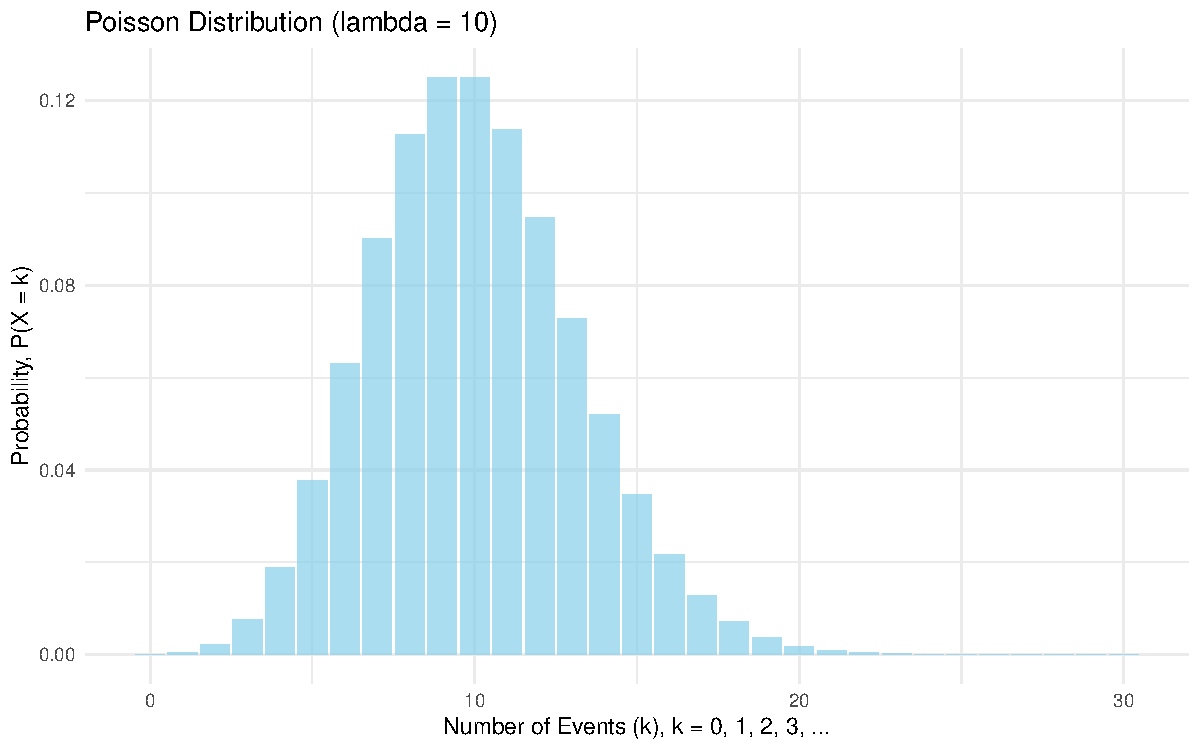
\includegraphics[width=10cm]{figure/unnamed-chunk-6-1} \end{center}

\begin{table}[!h]
\centering\centering
\resizebox{\ifdim\width>\linewidth\linewidth\else\width\fi}{!}{
\begin{tabular}[t]{ccccccccccccccc}
\toprule
\multicolumn{1}{c}{ } & \multicolumn{14}{c}{lambda} \\
\cmidrule(l{3pt}r{3pt}){2-15}
k & 0.1 & 0.2 & 0.3 & 0.4 & 0.5 & 0.6 & 0.7 & 0.8 & 0.9 & 1 & 1.5 & 2 & 2.5 & 3\\
\midrule
\cellcolor{gray!10}{0} & \cellcolor{gray!10}{0.905} & \cellcolor{gray!10}{0.819} & \cellcolor{gray!10}{0.741} & \cellcolor{gray!10}{0.670} & \cellcolor{gray!10}{0.607} & \cellcolor{gray!10}{0.549} & \cellcolor{gray!10}{0.497} & \cellcolor{gray!10}{0.449} & \cellcolor{gray!10}{0.407} & \cellcolor{gray!10}{0.368} & \cellcolor{gray!10}{0.223} & \cellcolor{gray!10}{0.135} & \cellcolor{gray!10}{0.082} & \cellcolor{gray!10}{0.050}\\
1 & 0.090 & 0.164 & 0.222 & 0.268 & 0.303 & 0.329 & 0.348 & 0.359 & 0.366 & 0.368 & 0.335 & 0.271 & 0.205 & 0.149\\
\cellcolor{gray!10}{2} & \cellcolor{gray!10}{0.005} & \cellcolor{gray!10}{0.016} & \cellcolor{gray!10}{0.033} & \cellcolor{gray!10}{0.054} & \cellcolor{gray!10}{0.076} & \cellcolor{gray!10}{0.099} & \cellcolor{gray!10}{0.122} & \cellcolor{gray!10}{0.144} & \cellcolor{gray!10}{0.165} & \cellcolor{gray!10}{0.184} & \cellcolor{gray!10}{0.251} & \cellcolor{gray!10}{0.271} & \cellcolor{gray!10}{0.257} & \cellcolor{gray!10}{0.224}\\
3 & 0.000 & 0.001 & 0.003 & 0.007 & 0.013 & 0.020 & 0.028 & 0.038 & 0.049 & 0.061 & 0.126 & 0.180 & 0.214 & 0.224\\
\cellcolor{gray!10}{4} & \cellcolor{gray!10}{0.000} & \cellcolor{gray!10}{0.000} & \cellcolor{gray!10}{0.000} & \cellcolor{gray!10}{0.001} & \cellcolor{gray!10}{0.002} & \cellcolor{gray!10}{0.003} & \cellcolor{gray!10}{0.005} & \cellcolor{gray!10}{0.008} & \cellcolor{gray!10}{0.011} & \cellcolor{gray!10}{0.015} & \cellcolor{gray!10}{0.047} & \cellcolor{gray!10}{0.090} & \cellcolor{gray!10}{0.134} & \cellcolor{gray!10}{0.168}\\
\addlinespace
5 & 0.000 & 0.000 & 0.000 & 0.000 & 0.000 & 0.000 & 0.001 & 0.001 & 0.002 & 0.003 & 0.014 & 0.036 & 0.067 & 0.101\\
\cellcolor{gray!10}{6} & \cellcolor{gray!10}{0.000} & \cellcolor{gray!10}{0.000} & \cellcolor{gray!10}{0.000} & \cellcolor{gray!10}{0.000} & \cellcolor{gray!10}{0.000} & \cellcolor{gray!10}{0.000} & \cellcolor{gray!10}{0.000} & \cellcolor{gray!10}{0.000} & \cellcolor{gray!10}{0.000} & \cellcolor{gray!10}{0.001} & \cellcolor{gray!10}{0.004} & \cellcolor{gray!10}{0.012} & \cellcolor{gray!10}{0.028} & \cellcolor{gray!10}{0.050}\\
7 & 0.000 & 0.000 & 0.000 & 0.000 & 0.000 & 0.000 & 0.000 & 0.000 & 0.000 & 0.000 & 0.001 & 0.003 & 0.010 & 0.022\\
\cellcolor{gray!10}{8} & \cellcolor{gray!10}{0.000} & \cellcolor{gray!10}{0.000} & \cellcolor{gray!10}{0.000} & \cellcolor{gray!10}{0.000} & \cellcolor{gray!10}{0.000} & \cellcolor{gray!10}{0.000} & \cellcolor{gray!10}{0.000} & \cellcolor{gray!10}{0.000} & \cellcolor{gray!10}{0.000} & \cellcolor{gray!10}{0.000} & \cellcolor{gray!10}{0.000} & \cellcolor{gray!10}{0.001} & \cellcolor{gray!10}{0.003} & \cellcolor{gray!10}{0.008}\\
9 & 0.000 & 0.000 & 0.000 & 0.000 & 0.000 & 0.000 & 0.000 & 0.000 & 0.000 & 0.000 & 0.000 & 0.000 & 0.001 & 0.003\\
\addlinespace
\cellcolor{gray!10}{10} & \cellcolor{gray!10}{0.000} & \cellcolor{gray!10}{0.000} & \cellcolor{gray!10}{0.000} & \cellcolor{gray!10}{0.000} & \cellcolor{gray!10}{0.000} & \cellcolor{gray!10}{0.000} & \cellcolor{gray!10}{0.000} & \cellcolor{gray!10}{0.000} & \cellcolor{gray!10}{0.000} & \cellcolor{gray!10}{0.000} & \cellcolor{gray!10}{0.000} & \cellcolor{gray!10}{0.000} & \cellcolor{gray!10}{0.000} & \cellcolor{gray!10}{0.001}\\
\bottomrule
\end{tabular}}
\end{table}

\newpage

\subsubsection{Table 6.2: (Continued) Poisson
Probabilities.}\label{table-6.2-continued-poisson-probabilities.}

\begin{table}[!h]
\centering\centering
\resizebox{\ifdim\width>\linewidth\linewidth\else\width\fi}{!}{
\begin{tabular}[t]{ccccccccccccccc}
\toprule
\multicolumn{1}{c}{ } & \multicolumn{14}{c}{lambda} \\
\cmidrule(l{3pt}r{3pt}){2-15}
k & 3.5 & 4 & 4.5 & 5 & 5.5 & 6 & 6.5 & 7 & 7.5 & 8 & 8.5 & 9 & 9.5 & 10\\
\midrule
\cellcolor{gray!10}{0} & \cellcolor{gray!10}{0.030} & \cellcolor{gray!10}{0.018} & \cellcolor{gray!10}{0.011} & \cellcolor{gray!10}{0.007} & \cellcolor{gray!10}{0.004} & \cellcolor{gray!10}{0.002} & \cellcolor{gray!10}{0.002} & \cellcolor{gray!10}{0.001} & \cellcolor{gray!10}{0.001} & \cellcolor{gray!10}{0.000} & \cellcolor{gray!10}{0.000} & \cellcolor{gray!10}{0.000} & \cellcolor{gray!10}{0.000} & \cellcolor{gray!10}{0.000}\\
1 & 0.106 & 0.073 & 0.050 & 0.034 & 0.022 & 0.015 & 0.010 & 0.006 & 0.004 & 0.003 & 0.002 & 0.001 & 0.001 & 0.000\\
\cellcolor{gray!10}{2} & \cellcolor{gray!10}{0.185} & \cellcolor{gray!10}{0.147} & \cellcolor{gray!10}{0.112} & \cellcolor{gray!10}{0.084} & \cellcolor{gray!10}{0.062} & \cellcolor{gray!10}{0.045} & \cellcolor{gray!10}{0.032} & \cellcolor{gray!10}{0.022} & \cellcolor{gray!10}{0.016} & \cellcolor{gray!10}{0.011} & \cellcolor{gray!10}{0.007} & \cellcolor{gray!10}{0.005} & \cellcolor{gray!10}{0.003} & \cellcolor{gray!10}{0.002}\\
3 & 0.216 & 0.195 & 0.169 & 0.140 & 0.113 & 0.089 & 0.069 & 0.052 & 0.039 & 0.029 & 0.021 & 0.015 & 0.011 & 0.008\\
\cellcolor{gray!10}{4} & \cellcolor{gray!10}{0.189} & \cellcolor{gray!10}{0.195} & \cellcolor{gray!10}{0.190} & \cellcolor{gray!10}{0.175} & \cellcolor{gray!10}{0.156} & \cellcolor{gray!10}{0.134} & \cellcolor{gray!10}{0.112} & \cellcolor{gray!10}{0.091} & \cellcolor{gray!10}{0.073} & \cellcolor{gray!10}{0.057} & \cellcolor{gray!10}{0.044} & \cellcolor{gray!10}{0.034} & \cellcolor{gray!10}{0.025} & \cellcolor{gray!10}{0.019}\\
\addlinespace
5 & 0.132 & 0.156 & 0.171 & 0.175 & 0.171 & 0.161 & 0.145 & 0.128 & 0.109 & 0.092 & 0.075 & 0.061 & 0.048 & 0.038\\
\cellcolor{gray!10}{6} & \cellcolor{gray!10}{0.077} & \cellcolor{gray!10}{0.104} & \cellcolor{gray!10}{0.128} & \cellcolor{gray!10}{0.146} & \cellcolor{gray!10}{0.157} & \cellcolor{gray!10}{0.161} & \cellcolor{gray!10}{0.157} & \cellcolor{gray!10}{0.149} & \cellcolor{gray!10}{0.137} & \cellcolor{gray!10}{0.122} & \cellcolor{gray!10}{0.107} & \cellcolor{gray!10}{0.091} & \cellcolor{gray!10}{0.076} & \cellcolor{gray!10}{0.063}\\
7 & 0.039 & 0.060 & 0.082 & 0.104 & 0.123 & 0.138 & 0.146 & 0.149 & 0.146 & 0.140 & 0.129 & 0.117 & 0.104 & 0.090\\
\cellcolor{gray!10}{8} & \cellcolor{gray!10}{0.017} & \cellcolor{gray!10}{0.030} & \cellcolor{gray!10}{0.046} & \cellcolor{gray!10}{0.065} & \cellcolor{gray!10}{0.085} & \cellcolor{gray!10}{0.103} & \cellcolor{gray!10}{0.119} & \cellcolor{gray!10}{0.130} & \cellcolor{gray!10}{0.137} & \cellcolor{gray!10}{0.140} & \cellcolor{gray!10}{0.138} & \cellcolor{gray!10}{0.132} & \cellcolor{gray!10}{0.123} & \cellcolor{gray!10}{0.113}\\
9 & 0.007 & 0.013 & 0.023 & 0.036 & 0.052 & 0.069 & 0.086 & 0.101 & 0.114 & 0.124 & 0.130 & 0.132 & 0.130 & 0.125\\
\addlinespace
\cellcolor{gray!10}{10} & \cellcolor{gray!10}{0.002} & \cellcolor{gray!10}{0.005} & \cellcolor{gray!10}{0.010} & \cellcolor{gray!10}{0.018} & \cellcolor{gray!10}{0.029} & \cellcolor{gray!10}{0.041} & \cellcolor{gray!10}{0.056} & \cellcolor{gray!10}{0.071} & \cellcolor{gray!10}{0.086} & \cellcolor{gray!10}{0.099} & \cellcolor{gray!10}{0.110} & \cellcolor{gray!10}{0.119} & \cellcolor{gray!10}{0.124} & \cellcolor{gray!10}{0.125}\\
11 & 0.001 & 0.002 & 0.004 & 0.008 & 0.014 & 0.023 & 0.033 & 0.045 & 0.059 & 0.072 & 0.085 & 0.097 & 0.107 & 0.114\\
\cellcolor{gray!10}{12} & \cellcolor{gray!10}{0.000} & \cellcolor{gray!10}{0.001} & \cellcolor{gray!10}{0.002} & \cellcolor{gray!10}{0.003} & \cellcolor{gray!10}{0.007} & \cellcolor{gray!10}{0.011} & \cellcolor{gray!10}{0.018} & \cellcolor{gray!10}{0.026} & \cellcolor{gray!10}{0.037} & \cellcolor{gray!10}{0.048} & \cellcolor{gray!10}{0.060} & \cellcolor{gray!10}{0.073} & \cellcolor{gray!10}{0.084} & \cellcolor{gray!10}{0.095}\\
13 & 0.000 & 0.000 & 0.001 & 0.001 & 0.003 & 0.005 & 0.009 & 0.014 & 0.021 & 0.030 & 0.040 & 0.050 & 0.062 & 0.073\\
\cellcolor{gray!10}{14} & \cellcolor{gray!10}{0.000} & \cellcolor{gray!10}{0.000} & \cellcolor{gray!10}{0.000} & \cellcolor{gray!10}{0.000} & \cellcolor{gray!10}{0.001} & \cellcolor{gray!10}{0.002} & \cellcolor{gray!10}{0.004} & \cellcolor{gray!10}{0.007} & \cellcolor{gray!10}{0.011} & \cellcolor{gray!10}{0.017} & \cellcolor{gray!10}{0.024} & \cellcolor{gray!10}{0.032} & \cellcolor{gray!10}{0.042} & \cellcolor{gray!10}{0.052}\\
\addlinespace
15 & 0.000 & 0.000 & 0.000 & 0.000 & 0.000 & 0.001 & 0.002 & 0.003 & 0.006 & 0.009 & 0.014 & 0.019 & 0.027 & 0.035\\
\cellcolor{gray!10}{16} & \cellcolor{gray!10}{0.000} & \cellcolor{gray!10}{0.000} & \cellcolor{gray!10}{0.000} & \cellcolor{gray!10}{0.000} & \cellcolor{gray!10}{0.000} & \cellcolor{gray!10}{0.000} & \cellcolor{gray!10}{0.001} & \cellcolor{gray!10}{0.001} & \cellcolor{gray!10}{0.003} & \cellcolor{gray!10}{0.005} & \cellcolor{gray!10}{0.007} & \cellcolor{gray!10}{0.011} & \cellcolor{gray!10}{0.016} & \cellcolor{gray!10}{0.022}\\
17 & 0.000 & 0.000 & 0.000 & 0.000 & 0.000 & 0.000 & 0.000 & 0.001 & 0.001 & 0.002 & 0.004 & 0.006 & 0.009 & 0.013\\
\cellcolor{gray!10}{18} & \cellcolor{gray!10}{0.000} & \cellcolor{gray!10}{0.000} & \cellcolor{gray!10}{0.000} & \cellcolor{gray!10}{0.000} & \cellcolor{gray!10}{0.000} & \cellcolor{gray!10}{0.000} & \cellcolor{gray!10}{0.000} & \cellcolor{gray!10}{0.000} & \cellcolor{gray!10}{0.000} & \cellcolor{gray!10}{0.001} & \cellcolor{gray!10}{0.002} & \cellcolor{gray!10}{0.003} & \cellcolor{gray!10}{0.005} & \cellcolor{gray!10}{0.007}\\
19 & 0.000 & 0.000 & 0.000 & 0.000 & 0.000 & 0.000 & 0.000 & 0.000 & 0.000 & 0.000 & 0.001 & 0.001 & 0.002 & 0.004\\
\addlinespace
\cellcolor{gray!10}{20} & \cellcolor{gray!10}{0.000} & \cellcolor{gray!10}{0.000} & \cellcolor{gray!10}{0.000} & \cellcolor{gray!10}{0.000} & \cellcolor{gray!10}{0.000} & \cellcolor{gray!10}{0.000} & \cellcolor{gray!10}{0.000} & \cellcolor{gray!10}{0.000} & \cellcolor{gray!10}{0.000} & \cellcolor{gray!10}{0.000} & \cellcolor{gray!10}{0.000} & \cellcolor{gray!10}{0.001} & \cellcolor{gray!10}{0.001} & \cellcolor{gray!10}{0.002}\\
21 & 0.000 & 0.000 & 0.000 & 0.000 & 0.000 & 0.000 & 0.000 & 0.000 & 0.000 & 0.000 & 0.000 & 0.000 & 0.000 & 0.001\\
\cellcolor{gray!10}{22} & \cellcolor{gray!10}{0.000} & \cellcolor{gray!10}{0.000} & \cellcolor{gray!10}{0.000} & \cellcolor{gray!10}{0.000} & \cellcolor{gray!10}{0.000} & \cellcolor{gray!10}{0.000} & \cellcolor{gray!10}{0.000} & \cellcolor{gray!10}{0.000} & \cellcolor{gray!10}{0.000} & \cellcolor{gray!10}{0.000} & \cellcolor{gray!10}{0.000} & \cellcolor{gray!10}{0.000} & \cellcolor{gray!10}{0.000} & \cellcolor{gray!10}{0.000}\\
23 & 0.000 & 0.000 & 0.000 & 0.000 & 0.000 & 0.000 & 0.000 & 0.000 & 0.000 & 0.000 & 0.000 & 0.000 & 0.000 & 0.000\\
\bottomrule
\end{tabular}}
\end{table}

\newpage

\subsubsection{Table 6.3: (Continued) Poisson
Probabilities.}\label{table-6.3-continued-poisson-probabilities.}

\begin{table}[!h]
\centering\centering
\resizebox{\ifdim\width>\linewidth\linewidth\else\width\fi}{!}{
\begin{tabular}[t]{ccccccccccccccc}
\toprule
\multicolumn{1}{c}{ } & \multicolumn{14}{c}{lambda} \\
\cmidrule(l{3pt}r{3pt}){2-15}
k & 11 & 12 & 13 & 14 & 15 & 16 & 17 & 18 & 19 & 20 & 25 & 30 & 40 & 50\\
\midrule
\cellcolor{gray!10}{0} & \cellcolor{gray!10}{0.000} & \cellcolor{gray!10}{0.000} & \cellcolor{gray!10}{0.000} & \cellcolor{gray!10}{0.000} & \cellcolor{gray!10}{0.000} & \cellcolor{gray!10}{0.000} & \cellcolor{gray!10}{0.000} & \cellcolor{gray!10}{0.000} & \cellcolor{gray!10}{0.000} & \cellcolor{gray!10}{0.000} & \cellcolor{gray!10}{0.000} & \cellcolor{gray!10}{0.000} & \cellcolor{gray!10}{0.000} & \cellcolor{gray!10}{0.000}\\
1 & 0.000 & 0.000 & 0.000 & 0.000 & 0.000 & 0.000 & 0.000 & 0.000 & 0.000 & 0.000 & 0.000 & 0.000 & 0.000 & 0.000\\
\cellcolor{gray!10}{2} & \cellcolor{gray!10}{0.001} & \cellcolor{gray!10}{0.000} & \cellcolor{gray!10}{0.000} & \cellcolor{gray!10}{0.000} & \cellcolor{gray!10}{0.000} & \cellcolor{gray!10}{0.000} & \cellcolor{gray!10}{0.000} & \cellcolor{gray!10}{0.000} & \cellcolor{gray!10}{0.000} & \cellcolor{gray!10}{0.000} & \cellcolor{gray!10}{0.000} & \cellcolor{gray!10}{0.000} & \cellcolor{gray!10}{0.000} & \cellcolor{gray!10}{0.000}\\
3 & 0.004 & 0.002 & 0.001 & 0.000 & 0.000 & 0.000 & 0.000 & 0.000 & 0.000 & 0.000 & 0.000 & 0.000 & 0.000 & 0.000\\
\cellcolor{gray!10}{4} & \cellcolor{gray!10}{0.010} & \cellcolor{gray!10}{0.005} & \cellcolor{gray!10}{0.003} & \cellcolor{gray!10}{0.001} & \cellcolor{gray!10}{0.001} & \cellcolor{gray!10}{0.000} & \cellcolor{gray!10}{0.000} & \cellcolor{gray!10}{0.000} & \cellcolor{gray!10}{0.000} & \cellcolor{gray!10}{0.000} & \cellcolor{gray!10}{0.000} & \cellcolor{gray!10}{0.000} & \cellcolor{gray!10}{0.000} & \cellcolor{gray!10}{0.000}\\
\addlinespace
5 & 0.022 & 0.013 & 0.007 & 0.004 & 0.002 & 0.001 & 0.000 & 0.000 & 0.000 & 0.000 & 0.000 & 0.000 & 0.000 & 0.000\\
\cellcolor{gray!10}{6} & \cellcolor{gray!10}{0.041} & \cellcolor{gray!10}{0.025} & \cellcolor{gray!10}{0.015} & \cellcolor{gray!10}{0.009} & \cellcolor{gray!10}{0.005} & \cellcolor{gray!10}{0.003} & \cellcolor{gray!10}{0.001} & \cellcolor{gray!10}{0.001} & \cellcolor{gray!10}{0.000} & \cellcolor{gray!10}{0.000} & \cellcolor{gray!10}{0.000} & \cellcolor{gray!10}{0.000} & \cellcolor{gray!10}{0.000} & \cellcolor{gray!10}{0.000}\\
7 & 0.065 & 0.044 & 0.028 & 0.017 & 0.010 & 0.006 & 0.003 & 0.002 & 0.001 & 0.001 & 0.000 & 0.000 & 0.000 & 0.000\\
\cellcolor{gray!10}{8} & \cellcolor{gray!10}{0.089} & \cellcolor{gray!10}{0.066} & \cellcolor{gray!10}{0.046} & \cellcolor{gray!10}{0.030} & \cellcolor{gray!10}{0.019} & \cellcolor{gray!10}{0.012} & \cellcolor{gray!10}{0.007} & \cellcolor{gray!10}{0.004} & \cellcolor{gray!10}{0.002} & \cellcolor{gray!10}{0.001} & \cellcolor{gray!10}{0.000} & \cellcolor{gray!10}{0.000} & \cellcolor{gray!10}{0.000} & \cellcolor{gray!10}{0.000}\\
9 & 0.109 & 0.087 & 0.066 & 0.047 & 0.032 & 0.021 & 0.014 & 0.008 & 0.005 & 0.003 & 0.000 & 0.000 & 0.000 & 0.000\\
\addlinespace
\cellcolor{gray!10}{10} & \cellcolor{gray!10}{0.119} & \cellcolor{gray!10}{0.105} & \cellcolor{gray!10}{0.086} & \cellcolor{gray!10}{0.066} & \cellcolor{gray!10}{0.049} & \cellcolor{gray!10}{0.034} & \cellcolor{gray!10}{0.023} & \cellcolor{gray!10}{0.015} & \cellcolor{gray!10}{0.009} & \cellcolor{gray!10}{0.006} & \cellcolor{gray!10}{0.000} & \cellcolor{gray!10}{0.000} & \cellcolor{gray!10}{0.000} & \cellcolor{gray!10}{0.000}\\
11 & 0.119 & 0.114 & 0.101 & 0.084 & 0.066 & 0.050 & 0.036 & 0.025 & 0.016 & 0.011 & 0.001 & 0.000 & 0.000 & 0.000\\
\cellcolor{gray!10}{12} & \cellcolor{gray!10}{0.109} & \cellcolor{gray!10}{0.114} & \cellcolor{gray!10}{0.110} & \cellcolor{gray!10}{0.098} & \cellcolor{gray!10}{0.083} & \cellcolor{gray!10}{0.066} & \cellcolor{gray!10}{0.050} & \cellcolor{gray!10}{0.037} & \cellcolor{gray!10}{0.026} & \cellcolor{gray!10}{0.018} & \cellcolor{gray!10}{0.002} & \cellcolor{gray!10}{0.000} & \cellcolor{gray!10}{0.000} & \cellcolor{gray!10}{0.000}\\
13 & 0.093 & 0.106 & 0.110 & 0.106 & 0.096 & 0.081 & 0.066 & 0.051 & 0.038 & 0.027 & 0.003 & 0.000 & 0.000 & 0.000\\
\cellcolor{gray!10}{14} & \cellcolor{gray!10}{0.073} & \cellcolor{gray!10}{0.090} & \cellcolor{gray!10}{0.102} & \cellcolor{gray!10}{0.106} & \cellcolor{gray!10}{0.102} & \cellcolor{gray!10}{0.093} & \cellcolor{gray!10}{0.080} & \cellcolor{gray!10}{0.065} & \cellcolor{gray!10}{0.051} & \cellcolor{gray!10}{0.039} & \cellcolor{gray!10}{0.006} & \cellcolor{gray!10}{0.001} & \cellcolor{gray!10}{0.000} & \cellcolor{gray!10}{0.000}\\
\addlinespace
15 & 0.053 & 0.072 & 0.088 & 0.099 & 0.102 & 0.099 & 0.091 & 0.079 & 0.065 & 0.052 & 0.010 & 0.001 & 0.000 & 0.000\\
\cellcolor{gray!10}{16} & \cellcolor{gray!10}{0.037} & \cellcolor{gray!10}{0.054} & \cellcolor{gray!10}{0.072} & \cellcolor{gray!10}{0.087} & \cellcolor{gray!10}{0.096} & \cellcolor{gray!10}{0.099} & \cellcolor{gray!10}{0.096} & \cellcolor{gray!10}{0.088} & \cellcolor{gray!10}{0.077} & \cellcolor{gray!10}{0.065} & \cellcolor{gray!10}{0.015} & \cellcolor{gray!10}{0.002} & \cellcolor{gray!10}{0.000} & \cellcolor{gray!10}{0.000}\\
17 & 0.024 & 0.038 & 0.055 & 0.071 & 0.085 & 0.093 & 0.096 & 0.094 & 0.086 & 0.076 & 0.023 & 0.003 & 0.000 & 0.000\\
\cellcolor{gray!10}{18} & \cellcolor{gray!10}{0.015} & \cellcolor{gray!10}{0.026} & \cellcolor{gray!10}{0.040} & \cellcolor{gray!10}{0.055} & \cellcolor{gray!10}{0.071} & \cellcolor{gray!10}{0.083} & \cellcolor{gray!10}{0.091} & \cellcolor{gray!10}{0.094} & \cellcolor{gray!10}{0.091} & \cellcolor{gray!10}{0.084} & \cellcolor{gray!10}{0.032} & \cellcolor{gray!10}{0.006} & \cellcolor{gray!10}{0.000} & \cellcolor{gray!10}{0.000}\\
19 & 0.008 & 0.016 & 0.027 & 0.041 & 0.056 & 0.070 & 0.081 & 0.089 & 0.091 & 0.089 & 0.042 & 0.009 & 0.000 & 0.000\\
\addlinespace
\cellcolor{gray!10}{20} & \cellcolor{gray!10}{0.005} & \cellcolor{gray!10}{0.010} & \cellcolor{gray!10}{0.018} & \cellcolor{gray!10}{0.029} & \cellcolor{gray!10}{0.042} & \cellcolor{gray!10}{0.056} & \cellcolor{gray!10}{0.069} & \cellcolor{gray!10}{0.080} & \cellcolor{gray!10}{0.087} & \cellcolor{gray!10}{0.089} & \cellcolor{gray!10}{0.052} & \cellcolor{gray!10}{0.013} & \cellcolor{gray!10}{0.000} & \cellcolor{gray!10}{0.000}\\
21 & 0.002 & 0.006 & 0.011 & 0.019 & 0.030 & 0.043 & 0.056 & 0.068 & 0.078 & 0.085 & 0.062 & 0.019 & 0.000 & 0.000\\
\cellcolor{gray!10}{22} & \cellcolor{gray!10}{0.001} & \cellcolor{gray!10}{0.003} & \cellcolor{gray!10}{0.006} & \cellcolor{gray!10}{0.012} & \cellcolor{gray!10}{0.020} & \cellcolor{gray!10}{0.031} & \cellcolor{gray!10}{0.043} & \cellcolor{gray!10}{0.056} & \cellcolor{gray!10}{0.068} & \cellcolor{gray!10}{0.077} & \cellcolor{gray!10}{0.070} & \cellcolor{gray!10}{0.026} & \cellcolor{gray!10}{0.001} & \cellcolor{gray!10}{0.000}\\
23 & 0.001 & 0.002 & 0.004 & 0.007 & 0.013 & 0.022 & 0.032 & 0.044 & 0.056 & 0.067 & 0.076 & 0.034 & 0.001 & 0.000\\
\cellcolor{gray!10}{24} & \cellcolor{gray!10}{0.000} & \cellcolor{gray!10}{0.001} & \cellcolor{gray!10}{0.002} & \cellcolor{gray!10}{0.004} & \cellcolor{gray!10}{0.008} & \cellcolor{gray!10}{0.014} & \cellcolor{gray!10}{0.023} & \cellcolor{gray!10}{0.033} & \cellcolor{gray!10}{0.044} & \cellcolor{gray!10}{0.056} & \cellcolor{gray!10}{0.080} & \cellcolor{gray!10}{0.043} & \cellcolor{gray!10}{0.002} & \cellcolor{gray!10}{0.000}\\
\addlinespace
25 & 0.000 & 0.000 & 0.001 & 0.002 & 0.005 & 0.009 & 0.015 & 0.024 & 0.034 & 0.045 & 0.080 & 0.051 & 0.003 & 0.000\\
\cellcolor{gray!10}{26} & \cellcolor{gray!10}{0.000} & \cellcolor{gray!10}{0.000} & \cellcolor{gray!10}{0.001} & \cellcolor{gray!10}{0.001} & \cellcolor{gray!10}{0.003} & \cellcolor{gray!10}{0.006} & \cellcolor{gray!10}{0.010} & \cellcolor{gray!10}{0.016} & \cellcolor{gray!10}{0.025} & \cellcolor{gray!10}{0.034} & \cellcolor{gray!10}{0.076} & \cellcolor{gray!10}{0.059} & \cellcolor{gray!10}{0.005} & \cellcolor{gray!10}{0.000}\\
27 & 0.000 & 0.000 & 0.000 & 0.001 & 0.002 & 0.003 & 0.006 & 0.011 & 0.017 & 0.025 & 0.071 & 0.066 & 0.007 & 0.000\\
\cellcolor{gray!10}{28} & \cellcolor{gray!10}{0.000} & \cellcolor{gray!10}{0.000} & \cellcolor{gray!10}{0.000} & \cellcolor{gray!10}{0.000} & \cellcolor{gray!10}{0.001} & \cellcolor{gray!10}{0.002} & \cellcolor{gray!10}{0.004} & \cellcolor{gray!10}{0.007} & \cellcolor{gray!10}{0.012} & \cellcolor{gray!10}{0.018} & \cellcolor{gray!10}{0.063} & \cellcolor{gray!10}{0.070} & \cellcolor{gray!10}{0.010} & \cellcolor{gray!10}{0.000}\\
29 & 0.000 & 0.000 & 0.000 & 0.000 & 0.000 & 0.001 & 0.002 & 0.004 & 0.008 & 0.013 & 0.054 & 0.073 & 0.014 & 0.000\\
\addlinespace
\cellcolor{gray!10}{30} & \cellcolor{gray!10}{0.000} & \cellcolor{gray!10}{0.000} & \cellcolor{gray!10}{0.000} & \cellcolor{gray!10}{0.000} & \cellcolor{gray!10}{0.000} & \cellcolor{gray!10}{0.001} & \cellcolor{gray!10}{0.001} & \cellcolor{gray!10}{0.003} & \cellcolor{gray!10}{0.005} & \cellcolor{gray!10}{0.008} & \cellcolor{gray!10}{0.045} & \cellcolor{gray!10}{0.073} & \cellcolor{gray!10}{0.018} & \cellcolor{gray!10}{0.001}\\
31 & 0.000 & 0.000 & 0.000 & 0.000 & 0.000 & 0.000 & 0.001 & 0.002 & 0.003 & 0.005 & 0.037 & 0.070 & 0.024 & 0.001\\
\cellcolor{gray!10}{32} & \cellcolor{gray!10}{0.000} & \cellcolor{gray!10}{0.000} & \cellcolor{gray!10}{0.000} & \cellcolor{gray!10}{0.000} & \cellcolor{gray!10}{0.000} & \cellcolor{gray!10}{0.000} & \cellcolor{gray!10}{0.000} & \cellcolor{gray!10}{0.001} & \cellcolor{gray!10}{0.002} & \cellcolor{gray!10}{0.003} & \cellcolor{gray!10}{0.029} & \cellcolor{gray!10}{0.066} & \cellcolor{gray!10}{0.030} & \cellcolor{gray!10}{0.002}\\
33 & 0.000 & 0.000 & 0.000 & 0.000 & 0.000 & 0.000 & 0.000 & 0.000 & 0.001 & 0.002 & 0.022 & 0.060 & 0.036 & 0.003\\
\cellcolor{gray!10}{34} & \cellcolor{gray!10}{0.000} & \cellcolor{gray!10}{0.000} & \cellcolor{gray!10}{0.000} & \cellcolor{gray!10}{0.000} & \cellcolor{gray!10}{0.000} & \cellcolor{gray!10}{0.000} & \cellcolor{gray!10}{0.000} & \cellcolor{gray!10}{0.000} & \cellcolor{gray!10}{0.001} & \cellcolor{gray!10}{0.001} & \cellcolor{gray!10}{0.016} & \cellcolor{gray!10}{0.053} & \cellcolor{gray!10}{0.042} & \cellcolor{gray!10}{0.004}\\
\addlinespace
35 & 0.000 & 0.000 & 0.000 & 0.000 & 0.000 & 0.000 & 0.000 & 0.000 & 0.000 & 0.001 & 0.011 & 0.045 & 0.049 & 0.005\\
\cellcolor{gray!10}{36} & \cellcolor{gray!10}{0.000} & \cellcolor{gray!10}{0.000} & \cellcolor{gray!10}{0.000} & \cellcolor{gray!10}{0.000} & \cellcolor{gray!10}{0.000} & \cellcolor{gray!10}{0.000} & \cellcolor{gray!10}{0.000} & \cellcolor{gray!10}{0.000} & \cellcolor{gray!10}{0.000} & \cellcolor{gray!10}{0.000} & \cellcolor{gray!10}{0.008} & \cellcolor{gray!10}{0.038} & \cellcolor{gray!10}{0.054} & \cellcolor{gray!10}{0.008}\\
37 & 0.000 & 0.000 & 0.000 & 0.000 & 0.000 & 0.000 & 0.000 & 0.000 & 0.000 & 0.000 & 0.005 & 0.031 & 0.058 & 0.010\\
\cellcolor{gray!10}{38} & \cellcolor{gray!10}{0.000} & \cellcolor{gray!10}{0.000} & \cellcolor{gray!10}{0.000} & \cellcolor{gray!10}{0.000} & \cellcolor{gray!10}{0.000} & \cellcolor{gray!10}{0.000} & \cellcolor{gray!10}{0.000} & \cellcolor{gray!10}{0.000} & \cellcolor{gray!10}{0.000} & \cellcolor{gray!10}{0.000} & \cellcolor{gray!10}{0.004} & \cellcolor{gray!10}{0.024} & \cellcolor{gray!10}{0.061} & \cellcolor{gray!10}{0.013}\\
39 & 0.000 & 0.000 & 0.000 & 0.000 & 0.000 & 0.000 & 0.000 & 0.000 & 0.000 & 0.000 & 0.002 & 0.019 & 0.063 & 0.017\\
\addlinespace
\cellcolor{gray!10}{40} & \cellcolor{gray!10}{0.000} & \cellcolor{gray!10}{0.000} & \cellcolor{gray!10}{0.000} & \cellcolor{gray!10}{0.000} & \cellcolor{gray!10}{0.000} & \cellcolor{gray!10}{0.000} & \cellcolor{gray!10}{0.000} & \cellcolor{gray!10}{0.000} & \cellcolor{gray!10}{0.000} & \cellcolor{gray!10}{0.000} & \cellcolor{gray!10}{0.001} & \cellcolor{gray!10}{0.014} & \cellcolor{gray!10}{0.063} & \cellcolor{gray!10}{0.021}\\
\bottomrule
\end{tabular}}
\end{table}

\end{document}
